\documentclass[12pt,openany,a4paper]{book}
\usepackage{amsmath}
\usepackage{amssymb}
\usepackage{graphics}	% if you want encapsulated PS figures.
\usepackage{graphicx}
\usepackage[colorlinks,allcolors=blue]{hyperref, xcolor} % must be bfore pgfplots
\usepackage{pgfplots} % must be after xcolor
\usepackage{colortbl}
\usepackage{float}
\usepackage{flafter}
\usepackage{pgfgantt}


% If you use a macro file called macros.tex :
% \input{macros}
% Note: The present document has its macros built in.

% Number subsections but not subsubsections:
\setcounter{secnumdepth}{2}
% Show subsections but not subsubsections in table of contents:
\setcounter{tocdepth}{2}

\pagestyle{headings}		% Chapter on left page, Section on right.
\raggedbottom

\setlength{\topmargin}		{-5mm}  %  25-5 = 20mm7
\setlength{\oddsidemargin}	{10mm}  % rhs page inner margin = 25+10mm
\setlength{\evensidemargin}	{0mm}   % lhs page outer margin = 25mm
\setlength{\textwidth}		{150mm} % 35 + 150 + 25 = 210mm
\setlength{\textheight}		{240mm} % 

\renewcommand{\baselinestretch}{1.2}	% Looks like 1.5 spacing.

% Stop figure/tables smaller than 3/4 page from appearing alone on a page:
\renewcommand{\textfraction}{0.25}
\renewcommand{\topfraction}{0.75}
\renewcommand{\bottomfraction}{0.75}
\renewcommand{\floatpagefraction}{0.75}

% THEOREM-LIKE ENVIRONMENTS:
\newtheorem{defn}	{Definition}	% cf. \dfn for cross-referencing
\newtheorem{theorem}	{Theorem}	% cf. \thrm for cross-referencing
\newtheorem{lemma}	{Lemma}		% cf. \lem for cross-referencing

% AIDS TO CROSS-REFERENCING (All take a label as argument):
\newcommand{\eref}[1] {(\ref{#1})}		% (...)
\newcommand{\eq}[1]   {Eq.\,(\ref{#1})}		% Eq.~(...)
\newcommand{\eqs}[2]  {Eqs.~(\ref{#1}) and~(\ref{#2})}
\newcommand{\dfn}[1]  {Definition~\ref{#1}}	% Definition~...
\newcommand{\thrm}[1] {Theorem~\ref{#1}}	% Theorem~...
\newcommand{\lem}[1]  {Lemma~\ref{#1}}		% Lemma~...
\newcommand{\fig}[1]  {Fig.\,\ref{#1}}		% Fig.~...
\newcommand{\tab}[1]  {Table~\ref{#1}}		% Table~...
\newcommand{\chap}[1] {Chapter~\ref{#1}}	% Chapter~...
\newcommand{\secn}[1] {Section~\ref{#1}}	% Section~...
\newcommand{\ssec}[1] {Subsection~\ref{#1}}	% Subsection~...

% AIDS TO FORMATTING:
\newcommand{\teq}[1]	{\mbox{$#1$}}	% in-Text EQuation (unbreakable)
\newcommand{\qed}	{\hspace*{\fill}$\bullet$}	% end of proof

% MATHEMATICAL TEMPLATES:
% Text or math mode:
\newcommand{\half}	{\ensuremath{\frac{1}{2}}}	% one-half
\newcommand{\halftxt}	{\mbox{$\frac{1}{2}$}}	  	% one-half, small
% Math mode only:
% N.B. Parentheses are ROUND; brackets are SQUARE!
\newcommand{\oneon}[1]	{\frac{1}{#1}}		  % reciprocal
\newcommand{\pow}[2]	{\left({#1}\right)^{#2}}  % Parenthesized pOWer
\newcommand{\bow}[2]	{\left[{#1}\right]^{#2}}  % Bracketed pOWer
\newcommand{\evalat}[2]	{\left.{#1}\right|_{#2}}  % EVALuated AT with bar
\newcommand{\bevalat}[2]{\left[{#1}\right]_{#2}}  % Bracketed EVALuated AT
% Total derivatives:
\newcommand{\sdd}[2]	{\frac{d{#1}}{d{#2}}}		    % Short
\newcommand{\sqdd}[2]	{\frac{d^2{#1}}{d{#2}^2}}	    % 2nd ("SQuared")
\newcommand{\ldd}[2]	{\frac{d}{d{#1}}\left({#2}\right)}  % Long paren'ed
\newcommand{\bdd}[2]	{\frac{d}{d{#2}}\left[{#2}\right]}  % long Bracketed
% Partial derivatives (same sequence as for total derivatives):
\newcommand{\sdada}[2]	{\frac{\partial {#1}}{\partial {#2}}}
\newcommand{\sqdada}[2]	{\frac{\partial ^{2}{#1}}{\partial {#2}^{2}}}
\newcommand{\ldada}[2]	{\frac{\partial}{\partial {#1}}\left({#2}\right)}
\newcommand{\bdada}[2]	{\frac{\partial}{\partial {#1}}\left[{#2}\right]}
\newcommand{\da}	{\partial}

% ORDINAL NUMBERS:
\newcommand{\ith}	{\ensuremath{i^{\rm th}}}
\newcommand{\jth}	{\ensuremath{j^{\rm th}}}
\newcommand{\kth}	{\ensuremath{k^{\rm th}}}
\newcommand{\lth}	{\ensuremath{l^{\rm th}}}
\newcommand{\mth}	{\ensuremath{m^{\rm th}}}
\newcommand{\nth}	{\ensuremath{n^{\rm th}}}

% SINUSOIDAL TIME AND SPACE-DEPENDENCY FACTORS:
\newcommand{\ejot}	{\ensuremath{e^{j\omega t}}}
\newcommand{\emjot}	{\ensuremath{e^{-j\omega t}}}

% UNITS (TEXT OR MATH MODE, WITH LEADING PADDING SPACE IF APPLICABLE):
% NB: These have not been tested since being modified for LaTeX2e.
\newcommand{\pack}	{\hspace{-0.08em}}
\newcommand{\Pack}	{\hspace{-0.12em}}
\newcommand{\mA}	{\ensuremath{\rm\,m\pack A}}
\newcommand{\dB}	{\ensuremath{\rm\,d\pack B}}
\newcommand{\dBm}	{\ensuremath{\rm\,d\pack B\pack m}}
\newcommand{\dBW}	{\ensuremath{\rm\,d\pack B\Pack W}}
\newcommand{\uF}	{\ensuremath{\rm\,\mu\pack F}}
\newcommand{\pF}	{\ensuremath{\rm\,p\pack F}}
\newcommand{\nF}	{\ensuremath{\rm\,n\pack F}}
\newcommand{\uH}	{\ensuremath{\rm\,\mu\pack H}}
\newcommand{\mH}	{\ensuremath{\rm\,m\pack H}}
\newcommand{\Hz}	{\ensuremath{\rm\,H\pack z}}
\newcommand{\kHz}	{\ensuremath{\rm\,k\pack H\pack z}}
\newcommand{\MHz}	{\ensuremath{\rm\,M\pack H\pack z}}
\newcommand{\GHz}	{\ensuremath{\rm\,G\pack H\pack z}}
\newcommand{\J}		{\ensuremath{\rm\,J}}
\newcommand{\kg}	{\ensuremath{\rm\,k\pack g}}
\newcommand{\K}		{\ensuremath{\rm\,K}}
\newcommand{\m}		{\ensuremath{\rm\,m}}
\newcommand{\cm}	{\ensuremath{\rm\,cm}}
\newcommand{\km}	{\ensuremath{\rm\,k\pack m}}
\newcommand{\mm}	{\ensuremath{\rm\,m\pack m}}
\newcommand{\nm}	{\ensuremath{\rm\,n\pack m}}
\newcommand{\um}	{\ensuremath{\rm\,\mu m}}
\newcommand{\Np}	{\ensuremath{\rm\,N\pack p}}
\newcommand{\s}		{\ensuremath{\rm\,s}}
\newcommand{\ms}	{\ensuremath{\rm\,m\pack s}}
\newcommand{\us}	{\ensuremath{\rm\,\mu s}}
\newcommand{\V}		{\ensuremath{\rm\,V}}
\newcommand{\mV}	{\ensuremath{\rm\,m\Pack V}}
\newcommand{\W}		{\ensuremath{\rm\,W}}
\newcommand{\mW}	{\ensuremath{\rm\,m\Pack W}}
\newcommand{\ohm}	{\ensuremath{\rm\,\Omega}}
\newcommand{\kohm}	{\ensuremath{\rm\,k\Omega}}
\newcommand{\Mohm}	{\ensuremath{\rm\,M\Omega}}
\newcommand{\degs}	{\ensuremath{\rm^{\circ}}}

% LaTeX run-time type-in command:
%
% \typein{Enter \protect\includeonly{...} command (or just type RETURN):}
%
% Uncommenting this command makes LaTeX prompt you for the \includeonly
% list.  At the prompt
%
%	\@typein=
%
% you type
%
%	\includeonly{chap1,chap2}
%
% to include the files chap1.tex and chap2.tex and omit any others.
% To include every \include file, just hit RETURN.
% If you are running LaTeX from xtexsh, you may need to click the mouse
% in the LaTeX window to position the cursor at the \@typein prompt.
\graphicspath{{/home/dmcinnes/git/thesis/thesis/thesis/images/}}
\begin{document}

\frontmatter
% By default, frontmatter has Roman page-numbering (i,ii,...).

\begin{titlepage}
\renewcommand{\baselinestretch}{1.0}
\begin{center}

\includegraphics{UQlogo}\\
\vspace*{35mm}
\Huge\bf
		A VERIFIED OCPP v2.01 SERVER\\
		FOR ELECTRIC VEHICLE CHARGER NETWORKS\\
\vspace{20mm}
\large\sl
		by\\
		DANIEL HUGH MCINNES
		\medskip\\
\rm
		School of Information Technology and Electrical Engineering,\\
		The University of Queensland.\\
\vspace{30mm}
		Submitted for the degree of\\
		Master of Engineering
		\smallskip\\
\normalsize
		in the field of Software Engineering
		\medskip\\
\large
		October 2019.		
\end{center}
\end{titlepage}

\cleardoublepage

\begin{flushright}
	Daniel McInnes\\
	s4231125@student.uq.edu.au\\
	\medskip
	\today
\end{flushright}
\begin{flushleft}
  Prof Amin Abbosh\\
  Acting Head of School\\
  School of Information Technology and Electrical Engineering\\
  The University of Queensland\\
  St Lucia, Q 4072\\
  \bigskip\bigskip
  Dear Professor Abbosh,

\medskip
In accordance with the requirements of the degree of Master of
Engineering in the division of 
Software Engineering,
I present the
following thesis entitled ``A Verified Server for an Electric Vehicle Charger Network''.  This work was performed under the supervision of A/Prof. Graeme Smith.
\medskip

I declare that the work submitted in this thesis is my own, except as
acknowledged in the text and footnotes, and has not been previously
submitted for a degree at The University of Queensland or any other
institution.

	Yours sincerely,\\
	\medskip
%	\emph{Author's Signature}\\
	\medskip
	Daniel McInnes.
\end{flushleft}

\cleardoublepage


\chapter{Acknowledgments}

I wish to acknowledge the support of my supervisor, Associate Professor Graeme Smith, whose expertise and assistance were greatly appreciated.
\cleardoublepage

\chapter{Abstract}

% Notice that all \include files are chapters -- a logical division.
% But not all chapters are \include files; some chapters are short
% enough to be in-lined in the main file.
Currently, networks of publicly available electric vehicle fast chargers communicate with servers using the Open Charge Point Protocol (OCPP). Ideally, the software running on these servers would be error free and never crash. Numerous software verification tools exist to prove desirable properties of the server software, such as functional correctness, the absence of race conditions, memory leaks, and certain runtime errors. I compare the different features of several verification tools, and choose one of them to partially implement an OCPP server.

\tableofcontents

\listoffigures
\addcontentsline{toc}{chapter}{List of Figures}

\listoftables
\addcontentsline{toc}{chapter}{List of Tables}

% If file los.tex begins with ``\chapter{List of Symbols}'':
% \include{los}

\cleardoublepage

\mainmatter
% By default, mainmatter has Arabic page-numbering (1,2,...).


% Chapters may be \include files, each beginning with a line like
%
%	\chapter{Title of chapter}
%
% e.g. if two chapter files were called intro.tex and theory.tex,
% we would say
%
%	\include{intro}
%	\include{theory}

\chapter{Introduction}



The International Energy Agency \cite{GlobalEVOutlook2019} reports that the number of publicly available fast chargers ($>$ 22kW) increased from 107\,650 in 2017 to 143\,502 in 2018.\\

\begin{figure}[htbp]
\caption{Publicly available fast chargers}


\begin{tikzpicture}
	\begin{axis}
	[
		ybar,
		scaled y ticks = false,
      		y tick label style={/pgf/number format/fixed,/pgf/number format/1000 sep = \thinspace},
		symbolic x coords={2007, 2008, 2009, 2010, 2011, 2012, 2013, 2014, 2015, 2016, 2017, 2018},
   	 	y label style={at={(axis description cs:-0.1,.5)},anchor=south},
		ylabel={Number of chargers},
		x label style={at={(axis description cs:0.5,-0.2)},anchor=north},
		xlabel={Year},
		x tick label style = {font = \small, text width = 1.7cm, align = center, rotate = 70, anchor = north east},
		xtick=data
	]
    	\addplot[ybar,fill=blue] coordinates {
        		(2007,42)
        		(2008,42)
        		(2009,47)
		(2010,372)
        		(2011,1356)
        		(2012,3332)
        		(2013,5044)
        		(2014,16762)
        		(2015,26784)
        		(2016,73851)
        		(2017,107650)
        		(2018,143502)
	};
\end{axis}
\end{tikzpicture}
\end{figure}


The Open Charge Alliance \cite{ocaappraisal} reports that more than 10\,000 charging stations\footnote{Note that a ``charging station'' may consist of multiple fast chargers, thus the disparity between 143\,502 ``fast chargers'' and ``more than 10\,000 charging stations''} in over 50 countries are managed using the OCPP protocol.


 
In this paper I investigate and compare the features of several different software verifiation tools and choose one to partially implement an OCPP server. The tools include Dafny, KeY, OpenJML, SPARK 2014, Spec\#, VCC, VeriFast, Viper, Whiley, and Why3.

The tools vary in what guarantees they provide. Desirable guarantees that I was interested in are: 
\label{criteria}
\begin{itemize}
	\item the absence of memory leaks
	\item the program should never access uninitialized memory (for example, should never read past the end of an array)
	\item the program should never crash or exit unexpectedly
	\item the tool should verify the absence of stack overflows, i.e. the program should be bounded in terms of memory (RAM) usage at runtime
	\item the program should verifiably meet its requirements. These requirements are typically in the form of preconditions and postconditions.
	\item the program should never exhibit undefined behaviour
	\item the program should constrain information flow, i.e. not leak sensitive information such as passwords
	\item The tool should be sound. Many of the tools claim to be sound ``modulo bugs in the tool'', and have lengthy lists of known bugs. 
\end{itemize}

\chapter{Prior Art}

Numerous software verification tools were considered for use in implementing the OCPP server. These tools include Dafny, KeY, OpenJML, SPARK 2014, Spec\#, VCC, Verifast, Viper, Whiley, and Why3. SPARK 2014 was found to best fulfill the criteria \ref{criteria}.

\section{Dafny}
	\subsection{Home Page}%	
		https://rise4fun.com/Dafny
	\subsection{Features}
		Dafny is both a language and a verifier \cite{LeinoK.R.M.2010DAap}. Dafny supports feature verification via preconditions, postconditions, loop invariants and loop variants. It uses the `Boogie' intermediate language and the Z3 theorem prover. The Dafny compiler produces executable files for the .NET platform \cite{dafny02}.
	\subsection{Soundness}
		Dafny is designed to be sound but incomplete, and is known to report errors on correct programs \cite{dafny01}.
	\subsection{Supported Platforms}
		Windows, Linux, OSX host, for a .NET target platform.
	\subsection{License Information}
		MIT.
	\subsection{Evidence of successful use in commercial software development}
		Internet searches failed to find any evidence of Dafny being used in commercial software development. 		
	\subsection{Existing Libraries}
		There is a `mathematics' library for Dafny.
		
	\subsection{Multithreaded Application Support}
		Internet searches failed to find evidence of multithreaded application support. 
		
	\subsection{Supported Languages}
		Dafny.

\section{KeY}
	\subsection{Home Page}%	
	https://www.key-project.org/
	\subsection{Features} 
		KeY offers functional verification for Java programs. The specifications are written as comments in JML in the Java source code. KeY is built on a formal logic called `Java Card DL', which is itself a first-order dynamic logic, and an extension of Hoare logic. It is targeted at JavaCard programs. 
	\subsection{Soundness} 
		KeY is thought to be sound. Internet searches failed to find examples of unsoundness.
	\subsection{Supported Platforms} 
		Windows, Linux, and OSX hosts, for a JVM target.
	\subsection{License Information} 
		GPL.		
	\subsection{Evidence of successful use in commercial software development} 
		Internet searches failed to find any evidence of KeY being used in commercial software development. 
	\subsection{Existing Libraries} 
		There are extensive libraries available for Java programs.
	\subsection{Multithreaded Application Support} 
		No.
	\subsection{Supported Languages} 
		Java.	










\section{OpenJML}
	\subsection{Home Page}%	
	http://www.openjml.org/
	\subsection{Features}
	OpenJML is a suite of tools for verifying Java programs that are annotated with JML statements. It is based on OpenJDKv1.8. It detects illegal memory access at compile time. It verifies preconditions and postconditions. It arguably guarantees the absence of undefined behaviour for single threaded applications. It does not constrain information flow.
	
	\subsection{Soundness}
	Yes
	\subsection{Supported Platforms}
	Windows, Linux, OSX.
	\subsection{License Information}
		GPLv2.
	\subsection{Evidence of successful use in commercial software development} 
		Internet searches failed to find any evidence of OpenJML being used in commercial software development. 

	\subsection{Existing Libraries} 
		There are extensive libraries available for Java programs.
	\subsection{Multithreaded Application Support}
	No.
	\subsection{Supported Languages}
	Java (only OpenJDK v1.8, may become unsupported in December 2020)

\section{SPARK 2014}
	SPARK 2014 is both a formally defined programming language and a set of verification tools. In typical use, a programmer writes SPARK code, which is compiled by the GNAT compiler, then analyzed by the GNATprove tool to produce numerous verification conditions. GNATprove uses Alt-Ergo, CVC4 and Z3 to prove the verification conditions.

	\subsubsection{Features}
	Formally verifies:
	\begin{itemize}
		\item information flow
		\item freedom from runtime errors, except `StorageError' (stack overflow / heap exhaustion)
		\item functional correctness
	\end{itemize}

	\subsubsection{Safety Standards}
		SPARK 2014 satisifes:
	\begin{itemize}
		\item DO-178B/C
		\item Formal Methods supplement DO-333
		\item CENELEC 51028
		\item IEC 61508
		\item DEFSTAN 00-56
	\end{itemize}

	\subsubsection{Soundness}
		SPARK is thought to be sound. Internet searches failed to find examples of unsoundness.

	\subsubsection{Supported Platforms}
		Windows, Linux, OSX.

	\subsubsection{License Information}
		Dual license:

		SPARK GPL is available for free from http://libre.adacore.com under the GPL.

		SPARK PRO is available under a commercial license from http://www.adacore.com.


	\subsubsection{Evidence of successful use in commercial software development}
	There is abundant evidence of the successful use of SPARK in high integrity software development. See: \cite{spark01}, \cite{spark02}, \cite{spark03}, \cite{spark04}, \cite{spark05}, \cite{spark06}, \cite{spark07}, \cite{spark08}, \cite{spark09}, \cite{spark10}, \cite{spark11}, \cite{spark12}, \cite{spark13}, \cite{spark14}, \cite{spark15}, \cite{spark16}, \cite{spark17}, \cite{spark18}, \cite{spark19}, \cite{spark20}, \cite{spark21}, \cite{spark22}, \cite{spark23}, \cite{spark24}, \cite{spark25}, \cite{spark26}, \cite{spark27}, \cite{spark28}, \cite{spark29}, \cite{spark30}, \cite{spark31}, \cite{spark32}, \cite{spark33}, \cite{spark34}, \cite{spark35}, \cite{spark36}, \cite{spark37}, \cite{spark38}, \cite{spark39}, \cite{spark40}, \cite{spark41}, \cite{spark42}, \cite{spark43}, \cite{spark44}, \cite{spark45}.
	
	
	Of particular relevance is the experience of the CubeSat Laboratory at Vermont Technical College\cite{sparkstudents}. Cubesats are small cubes launched into space with various sensors onboard, in this case without post-launch software update capabilities. This means the software must be fault free at the time of launch. The students (mostly third and fourth year undergraduates, with no prior knowledge of SPARK or Ada, and a high turnover rate) proved the software to be free of runtime errors. 14 Cubesats were launched in November 2013. Most were never heard from again, but the SPARK Cubesat worked for 2 years until it reentered Earth's atmosphere as planned in November 2015. 

	\subsubsection{Existing Libraries}
	SPARK has a minimal container library. SPARK interfaces easily with Ada, which has an extensive standard library.

	\subsubsection{Multithreaded Application Support}
	Unsupported.

	\subsubsection{Supported Languages}
	SPARK 2104 supports a subset of Ada 2012.


	See \cite[p.18]{McCormickJohnW.2015Bhia}

	``The following Ada 2012 features are not currently supported by Spark:

	Aliasing of names; no object may be referenced by multiple names

	Goto statements

	Expressions or functions with side effects

	Exception handlers

	Controlled types; types that provide fine control of object creation, assignment, and destruction

	Tasking/multithreading (will be included in future releases)''











\section{Spec\#}
	\subsection{Home Page}%	
	https://www.microsoft.com/en-us/research/project/spec/
	\subsection{Features}
		Spec\# consists of the Spec\# programming language, the Spec\# compiler, and the Spec\# static program verifier. The programming language is an extension of C\#, adding non-null types, checked exceptions, preconditions, postconditions, and object invariants \cite{spec01}. It uses Boogie for verification.
	\subsection{Soundness}
		Spec\# claims to be sound\cite{BarnettMike2005TSPS}.
	\subsection{Supported Platforms}
		Windows host platform, .NET target platform.
	\subsection{License Information}
		Internet searches failed to find Spec\# license information.
	\subsection{Evidence of successful use in commercial software development}
		Internet searches failed to find evidence of Spec\# being used in commercial software development.
	\subsection{Existing Libraries}
		Internet searches failed to find Spec\# libraries. However, Spec\# offers interoperability with the .NET platform, which has an extensive standard library, although the soundness of this library is not guaranteed.
	\subsection{Multithreaded Application Support}
		Yes\cite{spec01}.
	\subsection{Supported Languages}
		Spec\#.









\section{VCC}
	\subsection{Home Page}%	
		https://www.microsoft.com/en-us/research/project/vcc-a-verifier-for-concurrent-c/	
	\subsection{Features}
	VCC verifies preconditions and postconditions written in the form of special comments in the source code. 		It detects data races in multithreaded applications and illegal memory access at compile time. It does not 		guarantee the absence of undefined behaviour.

	\subsection{Soundness}
	Yes

	\subsection{Supported Platforms}
	Windows

	\subsection{License Information}
	%https://github.com/microsoft/vcc/blob/master/LICENSE
	MIT \cite{vcc01}

	\subsection{Evidence of successful use in commercial software development}
		VCC has been used successfully in at least one major commercial project, the verification of the Microsoft Hypervisor, the virtualization kernel of Hyper-V \cite{vcc2}.

	\subsection{Existing Libraries}
		Internet searches failed to find libraries verified with VCC. However, applications written with VCC can link against unverified libraries, effectively giving access to extensive library support.

	\subsection{Multithreaded Application Support}
	Yes

	\subsection{Supported Languages}
	C




\section{Verifast}
	\subsection{Home Page}%	
	https://github.com/verifast/verifast

	\subsection{Features}
	Verifast verifies preconditions, and postconditions in the form of special comments in the source code.
	It detects race conditions in multithreaded applications. It does not guarantee the absence of undefined behaviour, or verify the absence of stack overflows.	
	
	\subsection{Soundness}
	No, see https://github.com/verifast/verifast/blob/master/soundness.md
	\subsection{Supported Platforms}
	Windows, Linux, OSX.

	\subsection{License Information} 
	MIT \cite {verifastlicense}.
	\subsection{Evidence of successful use in commercial software development}
	There is evidence of some use in industrial applications\cite{PhilippaertsPieter2014SvwV}.
	\subsection{Existing Libraries}
		Internet searches failed to find libraries verified by / written with VeriFast annotations. However, applications written with VeriFast can link against unverified libraries, effectively gaining access to extensive library support.
	\subsection{Multithreaded Application Support}
	Yes.
	\subsection{Supported Languages}
	C, Java









\section{Viper}
	\subsection{Home Page}%	
https://www.pm.inf.ethz.ch/research/viper.html
	\subsection{Features}
		Viper consists of the Viper intermediate verification language, automatic verifiers, and example front end tools \cite{viper01}. It is more of a tool for creating other verification tools than a tool for verifying software. In practice, a developer would write code in Python and use the `Nagini' front end (based on Viper) to verify the code \cite{Eilers2018NaginiAS}. A corresponding front end for Rust exists, `Prusti' \cite{AstrauskasMuellerPoliSummers19}.
	\subsection{Soundness}
		Yes.
	\subsection{Supported Platforms}
		Windows, MacOS, Linux\cite{JuhaszUri2014VAVI}.
	\subsection{License Information}
	https://bitbucket.org/viperproject/carbon/src/default/LICENSE.txt
		Mozilla Public License Version 2.0\cite{viperlicense}
	\subsection{Evidence of successful use in commercial software development}
		Internet searches failed to find evidence of Viper being used in commercial software development.
	\subsection{Existing Libraries}
		Internet searches failed to find libraries verified by Viper front ends. However, applications written with these front ends can link against unverified libraries, effectively gaining access to extensive library support.
	\subsection{Multithreaded Application Support}
	Yes.
	\subsection{Supported Languages}
	Python, Rust, Java, OpenCL, Chalice.





\section{Whiley}
	\subsection{Home Page}
	http://whiley.org/
	
	\subsection{Features}
	Whiley consists of the Whiley language, the Whiley Build System, the Whiley Compiler, the Whiley Intermediate Language, the Whiley-2-Java Compiler, the Whiley-2-C Compiler, and the Whiley Constraint Solver\cite{10.1007/978-3-319-02654-1_13}. 
	
	Whiley uses a variant of first-order logic called the Whiley Assertion Language for verification.
	
	In typical use, a developer will write source code in Whiley, build with the Whiley Build system, and execute the resulting Java class file on the JVM.  

	\subsection{Soundness}
	Internet searches did not find evidence to indicate that Whiley is unsound.
	\subsection{Supported Platforms}
	JVM.
	\subsection{License Information}
	BSD.
	\subsection{Evidence of successful use in commercial software development}
		Internet searches failed to find evidence of Whiley being used in commercial software development.
	\subsection{Existing Libraries}
		Internet searches failed to find libraries verified by Whiley. However, applications written with Whiley can link against unverified Java functions, effectively gaining access to extensive library support.
	\subsection{Multithreaded Application Support}
	No.
	\subsection{Supported Languages}
	Whiley. The Whiley-2-Java Compiler (WyJC) can convert verified Whiley programs into JVM class files. Whiley can import Java functions, and export Whiley functions for use in Java programs.






\section{Why3}
	\subsection{Home Page}
	http://why3.lri.fr/
	\subsection{Features}
	The Why3 deductive program verification platform includes the WhyML language, a standard library of logical theories, and basic programming data structures\cite{why3homepage}. In typical use, a developer will write software in WhyML, and get correct-by-construction OCaml programs through an automated extraction mechanism. It verifies preconditions and postconditions.
	
	WhyML is also used by numerous popular verification tools (FramaC, SPARK2014, Krakatoa) as an intermediate language for verification of C, Java and Ada programs.
	\subsection{Soundness}
	Yes.
	\subsection{Supported Platforms}
	Windows, Linux, OSX. Why3 is distributed as a Debian package and as an OPAM package.
	
	\subsection{License Information}
	GNU LGPL 2.1.
	\subsection{Evidence of successful use in commercial software development}
		Internet searches failed to find evidence of WhyML being used in commercial software development. However, there are countless cases of commercial software development using WhyML as an intermediate language, as it is used by FramaC, SPARK, and others.
 
	\subsection{Existing Libraries}
	Why3 comes with a standard library of logical theories and basic programming data structures.
	\subsection{Multithreaded Application Support}
	No.
	\subsection{Supported Languages}
	WhyML.

\section{Conclusion of Review of Background and Associated Work}
Based on the properties of the verification tools available, it has been decided to use SPARK 2014 for the implementation and verification of the OCPP server. It has wide use in industry, which gives me confidence that it is a practical choice. It verifies all of the properties that are important to me, and has good library support.


%\section{Summary of Verification Tool Features}
%
%\begin{tabular}{ |p{1.3cm}||p{1.3cm}|p{1.5cm}|p{0.9cm}| p{0.9cm}|p{0.9cm}|p{1.4cm}|p{1.3cm}|p{1cm}| p{1cm}| }
% \hline
% \multicolumn{9}{|c|}{Features} \\
% \hline
 
%Tool & 
%\tiny No memory leaks & 
%\tiny Never accesses uninitialized memory & 
%\tiny Never crashes &
%\tiny Bounded RAM &
%\tiny Never hang &
%\tiny Proves Functional Correctness &
%\tiny No undefined behaviour &
%\tiny No data leak 
%\\
% \hline
%Dafny 		& \cellcolor{red} & \cellcolor{red}& \cellcolor{red} \ref{dafnybug1} %& \cellcolor{red} & \cellcolor{red} & \cellcolor{green} & \cellcolor{red} %\ref{unproven}  & \cellcolor{red} \ref{dafnybug2} \\
% \hline
%JML & 
%	\cellcolor{red}  & 
%	\cellcolor{green} & 
%	?& 
%	?& 
%	?& 
%	?& 
%	?& 
%	?\\
% \hline
%KeY & 
%	? & 
%	? & 
%	?& 
%	?& 
%	?& 
%	?& 
%	?& 
%	?\\
% \hline
%SPARK		& ? & ? & ?& ?& ?& ?& ?& ?\\
% \hline
%Spec \#		& ? & ? & ?& ?& ?& ?& ?& ?\\
% \hline
%Verifast& ? & ? & ?& ?& ?& ?& ?& ?\\
% \hline
%VCC& ? & ? & ?& ?& ?& ?& ?& ?\\
% \hline
%Viper& ? & ? & ?& ?& ?& ?& ?& ?\\
% \hline
%Whiley& ? & ? & ?& ?& ?& ?& ?& ?\\
% \hline
%Why3& ? & ? & ?& ?& ?& ?& ?& ?\\
% \hline
%\end{tabular}

%\label{unproven} Internet searches failed to find evidence that this is supported.










\chapter{OCPP Server Implementation}
\section{OCPP Overview}
An OCPP server acts as a websocket server. There are typically many individual charging stations, which act as websocket clients. The clients establish a websocket connection with the server, and once this is complete, JSON formatted packets are exchanged between the client and the server.
\begin{center}
\begin{figure}[htbp]
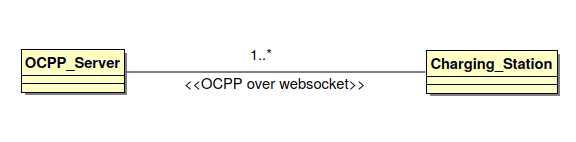
\includegraphics[width=\linewidth]{ocppOverview.png}
\caption{OCPP overview.}
\end{figure}

\end{center}


\section{Minimal OCPP implementation}
The OCPP protocol supports many use cases which are not required for a basic implementation. The following table \cite{ocpp} shows a minimal subset of OCPP messages required to support basic functionality.\\
\begin{center}
\begin{table}[htp]
\caption{Use cases for a basic implementation}
\begin{tabular}{ |p{5cm}|p{3cm}|p{4cm}|p{2cm}|}
 \hline
Functionality & 
Use Case & 
Messages
\\
 \hline
Booting a charge station& B01 - B04& BootNotification \\
 \hline
Configuring a charge station & B05-B07 & SetVariables, GetVariables, GetReportBase \\
 \hline
Resetting a charge station& B11-B12 & Reset \\
 \hline
Authorization Options& One of C01, C02, C04 & Authorize\\
 \hline
Transaction Mechanism & E01 (one of S1-S6), E02-E03,
E05, E06 (one of S1-S6), E07-
E08, One of E09-E10, E11-E13 & TransactionEvent \\
 \hline
Availability& G01, G03-G04& ChangeAvailability, StatusNotification\\
 \hline
Monitoring Events& G05, N07 & NotifyEvent\\
 \hline
Meter Values & J02 & TransactionEvent\\
 \hline
Data Transfer& P01-P02 & DataTransfer\\
 \hline
\end{tabular}
\end{table}
\end{center}

\subsection{Boot Notification Discussion}
To understand what interesting software properties may be proved, we will walk through a typical `BootNotification' sequence.\\

Whenever a charger is powered on in the field, it establishes a websocket connection with the server, and sends a `BootNotificationRequest' packet to announce itself. A high level view of a typical boot notification sequence is given in figure \ref{fig:SD-B01}.

	\begin{center}
		\begin{figure}[H]
			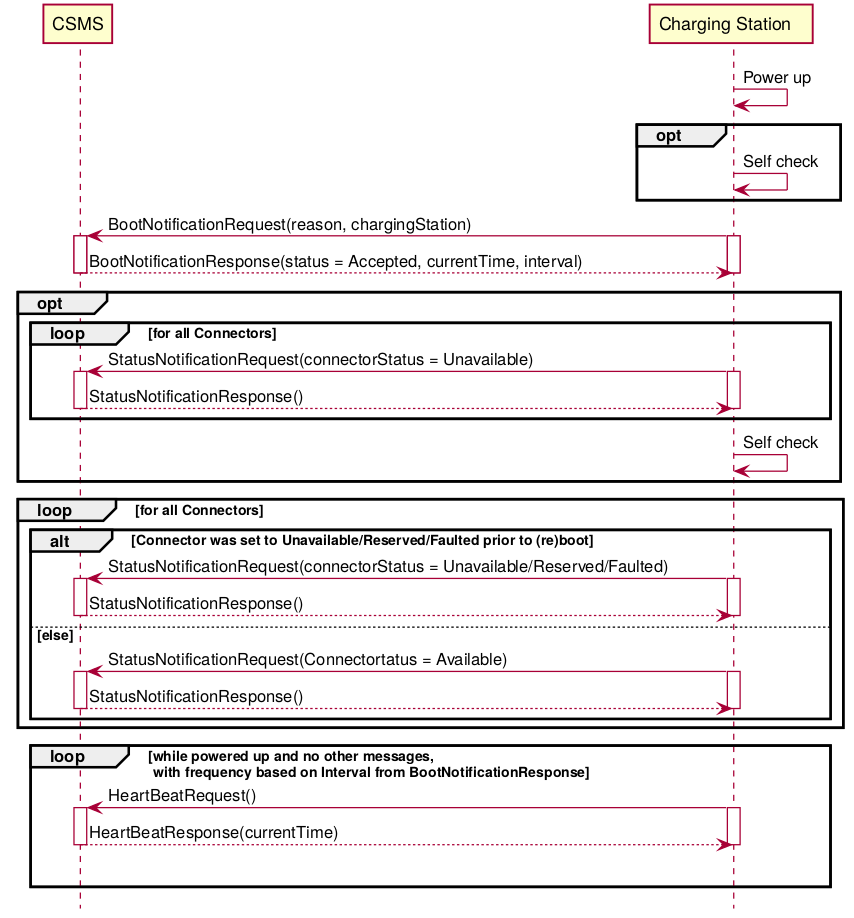
\includegraphics[width=\linewidth]{SD-B01}
			\caption{Cold Booting a Charging Station \cite{ocpp2b}.}
			\label{fig:SD-B01}
		\end{figure}
	\end{center}
	
The `BootNotificationRequest' packet contains information describing the charger. If the server recognises the charger, it returns a `BootNotificationResponse' message with a status of `Accepted'. The contents of these packets is described in figure \ref{fig:CDBootNotification}.

	\begin{center}
		\begin{figure}[H]
			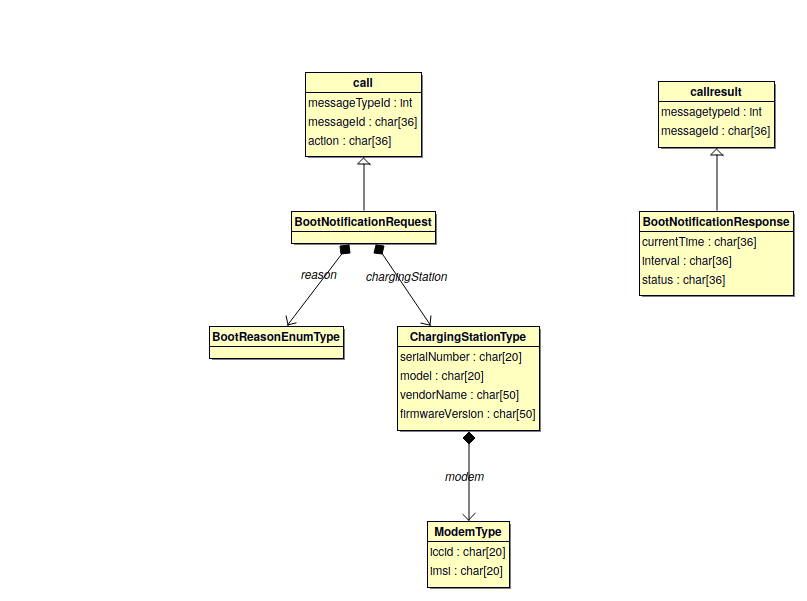
\includegraphics[width=\linewidth]{CDBootNotification}
			\caption{`Boot Notification' class diagram}
			\label{fig:CDBootNotification}
		\end{figure}
	\end{center}
	
Note that figure \ref{fig:CDBootNotification} is a UML class diagram, the different arrow types have special meanings. The `BootNotificationRequest' class inherits from the `call' class, and has a member variable called `reason' of class `BootReasonEnumType'. It also has a member variable called `chargingStation' of class `ChargingStationType', which in turn has a member variable called `modem' of class `ModemType'.

\pagebreak
The `BootNotificationRequest' packet arrives at the server as a big blob of text, as follows:
\begin{verbatim}
[2,	        // `2' indicates that this is a `request'
"19223202",// this is the message ID, and associates requests with responses
"BootNotification", // the `action'
{
   "chargingStation":
   {
      "serialNumber": "00000000000000000001",
      "model": "SingleSocketCharger",
      "modem":
      {
         "iccid": "01234567890123456789",
         "imsi": "01234567890123456789"
      },
      "vendorName": "VendorX",
      "firmwareVersion": "01.23456789"
   },
   "reason":"PowerUp"
}
]
\end{verbatim}

The server's job is to correctly parse this text, determine what kind of packet it is, and respond appropriately. In this example, the server converts the blob of incoming text into a `BootNotificationRequest' packet, builds a `BootNotificationResponse' packet, converts it to a blob of text, and sends it back over the websocket to the charger. The reponse looks like this:

\begin{verbatim}
[3,// `3' indicates that this is a `response'
"19223202",// this responds to request "19223202"
{
    "currentTime": "2013-02-01T20:53:32.486Z",
    "interval":  300,
    "status":"Accepted"
}
]
\end{verbatim}

\pagebreak

\subsection{OCPP message types}

Valid OCPP message types are either CALL, CALLRESULT, or CALLERROR.

\subsubsection{CALL}
A CALL consists of 4 parts, as described in \ref{tab:CALL}

\begin{table}[htp]
\begin{tabular}{ |p{3cm}|p{2.5cm}|p{9cm}| }
 \hline
\textbf{Field} & \textbf{Data Type} & \textbf{Meaning}
\\
 \hline MessageTypeId & Integer (=2)& This is a Message Type Number which is used to identify the type of the message.\\
 \hline MessageId & string[36] & This is a unique identifier that will be used to match request and result.\\
 \hline Action & string[36] & The name of the remote procedure or action. This field SHALL contain a case-sensitive string.
The field SHALL contain the OCPP Message name without the "Request" suffix. For example: For
a "BootNotificationRequest", this field shall be set to "BootNotification".\\
 \hline Payload & JSON & JSON Payload of the action.\\
 \hline
\end{tabular}
\caption{CALL message type \cite{ocpp4}}
\label{tab:CALL}
\end{table}


\subsubsection{CALLRESULT}
A CALL consists of 4 parts, as described in \ref{tab:CALLRESULT}

\begin{table}[H]
\begin{tabular}{ |p{3cm}|p{2.5cm}|p{9cm}| }
 \hline
\textbf{Field} & \textbf{Data Type} & \textbf{Meaning}
\\
 \hline MessageTypeId & Integer (=3) & This is a Message Type Number which is used to identify the type of the message.\\
 \hline MessageId & string[36] & This must be the exact same ID that is in the call request so that the recipient can match request and result.\\
 \hline Payload & JSON & JSON Payload of the action.\\
 \hline
\end{tabular}
\caption{CALLRESULT message type \cite{ocpp4}}
\label{tab:CALLRESULT}
\end{table}


\subsubsection{CALLERROR}
The CALLERROR message is only used when an error occurs during message transport, or in response to an invalid OCPP message. A CALL consists of 5 parts, as described in \ref{tab:CALLERROR}. 
\begin{table}[htp]
\begin{tabular}{ |p{3cm}|p{2.5cm}|p{9cm}| }
 \hline
\textbf{Field} & \textbf{Data Type} & \textbf{Meaning}
\\
 \hline MessageTypeId & Integer (=4)& This is a Message Type Number which is used to identify the type of the message.\\
 \hline MessageId & string[36] & This must be the exact same ID that is in the call request so that the recipient can match request and result.\\
 \hline Action & string[36] & The name of the remote procedure or action. This field SHALL contain a case-sensitive string.
The field SHALL contain the OCPP Message name without the "Request" suffix. For example: For
a "BootNotificationRequest", this field shall be set to "BootNotification".\\
 \hline Payload & JSON & JSON Payload of the action.\\
 \hline
\end{tabular}
\caption{CALLERROR message type \cite{ocpp4}}
\label{tab:CALLERROR}
\end{table}


\subsection{Implementation}
The sequence diagram \ref{fig:SDBootNotification} describes the typical sequence of events that occurs when a charger is powered on, boots up and connects to a server. Prior to the charger booting, the charger is enrolled on the server. The server maintains a list of known chargers. Only chargers on this list may successfully start an OCPP session.\\
Once a charger powers up, it establishes a websocket connection with the server and communicates with OCPP packets over this link. The first OCPP message the charger sends is a `BootNotificationRequest'.\\
When the server receives a blob of text, it arrives in a function called `ReceivePacket'.

\pagebreak
\subsection{`Server.ReceivePacket' Function}

\begin{verbatim}
   procedure ReceivePacket(theServer: in out ocpp.server.T;
                           msg: in NonSparkTypes.packet.Bounded_String;
                           response: out NonSparkTypes.packet.Bounded_String;
                           valid: out Boolean)
     with
       Global => null,
       Annotate => (GNATprove, Terminating),
       Depends => (
                   valid => (msg),
                   response => (msg, theServer),
                   theServer => (msg, theServer)
                  );
\end{verbatim}

\subsubsection{Global Data Dependencies}
The line `$Global \Rightarrow null$' specifies that the procedure may not modify any global variables. 
\subsubsection{`Annotate' section}
By default, GNATprove does not prove termination of subprograms. The line `$Annotate \Rightarrow (GNATprove, Terminating)$' specifies that the procedure must terminate, i.e. can never enter an endless loop. 
\subsubsection{`Depends' section}
The `Depends' clause means that:
\begin{itemize}
\item the final value of `valid' depends only on `msg'. It makes sense that the validity of an OCPP packet depends only on the content of the message, and is independent of the state of the server.
\item the final value of `response' depends on `msg' and on `theServer'. It makes intuitive sense that the response depends on what the request was. It may not be immediately obvious why the response should depend on the state of the server, until we consider that the server maintains a list of known chargers, and will respond to BootNotificationRequests with a `Rejected' status for unknown chargers.
\item the final value of `theServer' depends on the initial state of `theServer' and on `msg'. 
\end{itemize}

GNATprove reports an error if any of these specifications are not met by the implementation.\\


The first thing the function `ReceivePacket' does is parse the `MessageType', as seen in \ref{fig:SDBootNotification}. 

	\begin{center}
		\begin{figure}[H]
			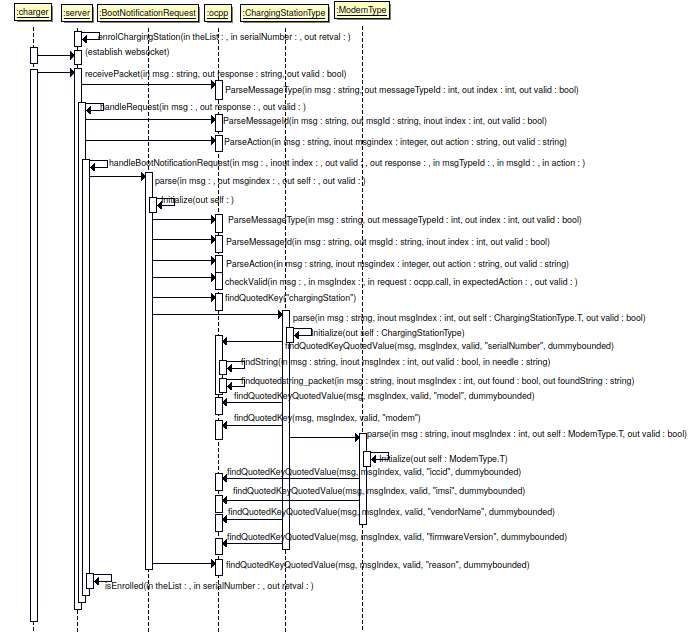
\includegraphics[width=\linewidth]{SDBootNotification}
			\caption{Cold Booting a Charging Station \cite{ocpp2b}.}
			\label{fig:SDBootNotification}
		\end{figure}
	\end{center}

\pagebreak
\subsection{`OCPP.ParseMessageType' Function}
\begin{verbatim}

   procedure ParseMessageType(msg:   in  NonSparkTypes.packet.Bounded_String;
                              messagetypeid : out integer;-- eg. 2
                              index: in out Integer;
                              valid: out Boolean)
     with  Global => null,
     Annotate => (GNATprove, Terminating),
     Post => (if valid = true then 
                (messagetypeid = 2 or messagetypeid = 3 or messagetypeid = 4)
              and
                (index < NonSparkTypes.packet.Length(msg))
             );
\end{verbatim}
\subsubsection{Global Data Dependencies}
The line `$Global \Rightarrow null$' specifies that the procedure may not modify any global variables. 
\subsubsection{`Annotate' section}
By default, GNATprove does not prove termination of subprograms. The line `$Annotate \Rightarrow (GNATprove, Terminating)$' specifies that the procedure must terminate, i.e. can never enter an endless loop. 
\subsubsection{`Post' section}
The `Post' clause means that:
\begin{itemize}
\item if the function returns `valid = true', then the `messagetypeid' must be one of the valid OCPP message types, i.e. 2, 3 or 4.
\item if the function returns `valid = true', then the `index' must not have moved past the end of `msg'. This postcondition is included as a sanity check. 
\end{itemize}

GNATprove reports an error if any of these specifications are not met by the implementation.\\

Once we have successfully parsed the message type, we know whether it is a `request' or a `response'. In this example, the server has received a `BootNotificationRequest', so we pass the message to `HandleRequest' for further parsing.

\subsection{`Server.HandleRequest' Function}
\begin{verbatim}
   procedure HandleRequest(theServer: in ocpp.server.T;
                           msg: in NonSparkTypes.packet.Bounded_String;
                           msgindex: in out Integer;
                           response: out NonSparkTypes.packet.Bounded_String;
                           valid: out Boolean)
     with
       global => null,
       Annotate => (GNATprove, Terminating),
       Depends => (
                   valid => (msg, msgindex),
                   msgindex => (msg, msgindex),
                   response => (msg, msgindex, theServer)
                  ),
       Post => (if valid = true then msgindex <= NonSparkTypes.packet.Length(msg));
   
\end{verbatim}
\subsubsection{`Global' section}
The line `$Global \Rightarrow null$' means that the procedure does not modify any global state.
\subsubsection{`Annotate' section}
By default, GNATprove does not prove termination of subprograms. The line `$Annotate \Rightarrow (GNATprove, Terminating)$' specifies that the procedure must terminate, i.e. can never enter an endless loop. 
\subsubsection{`Depends' section}
\begin{itemize}
\item The final value of `valid' depends only on `msg' and `msgindex'. The reason `valid' depends on `msgindex' is that if the index was already pointing at the end of the message, there would not be enough information left to construct a valid request.
\item The final value of `msgindex' depends only on `msg' and `msgindex'. This makes sense, as if the message was invalid, the function will return early, without parsing much of the message, thus affecting the final value of `index'. The reason the final value of `msgindex' depends on the initial value of `msgindex' is that if the index was already pointing at the end of the message, the function would return without advancing `msgindex' through the message.
\item The value of `response' depends on `msg', `msgindex' and `theServer'. 
\end{itemize}
\subsubsection{`Post' section}
The `Post' clause means that:
\begin{itemize}
\item if the function returns `valid = true', then the `index' must not have moved past the end of `msg'. This postcondition is included as a sanity check. 
\end{itemize}

GNATprove reports an error if any of these specifications are not met by the implementation.\\


The body of `HandleRequest()' calls `ParseAction' to determine what kind of request it is.

\subsection{`OCPP.ParseAction' Function}
\begin{verbatim}
   procedure ParseAction(msg:   in  NonSparkTypes.packet.Bounded_String;
                         msgindex: in out Integer;
                         action : out NonSparkTypes.action_t.Bounded_String;
                         valid: out Boolean
                        )
     with  Global => null,
     Annotate => (GNATprove, Terminating),
     Post => (if valid = true 
                then 
                  (msgindex < NonSparkTypes.packet.Length(msg))
             );

   
\end{verbatim}
\subsubsection{`Global' section}
The line `$Global \Rightarrow null$' means that the procedure does not modify any global state.
\subsubsection{`Annotate' section}
By default, GNATprove does not prove termination of subprograms. The line `$Annotate \Rightarrow (GNATprove, Terminating)$' specifies that the procedure must terminate, i.e. can never enter an endless loop. 
\subsubsection{`Depends' section}
\begin{itemize}
\item The final value of `valid' depends only on `msg' and `index'. The reason `valid' depends on `index' is that if the index was already pointing at the end of the message, there would not be enough information left to construct a valid request.
\item The final value of `index' depends only on `msg' and `index'. This makes sense, as if the message was invalid, the function will return early, without parsing much of the message, thus affecting the final value of `index'. The reason the final value of `index' depends on the initial value of `index' is that if the index was already pointing at the end of the message, the function would return without advancing `index' through the message.
\item The value of `response' depends on `msg', `index' and `theServer'. 
\end{itemize}
\subsubsection{`Post' section}
The `Post' clause means that:
\begin{itemize}
\item if the function returns `valid = true', then the `index' must not have moved past the end of `msg'. This postcondition is included as a sanity check. 
\end{itemize}

GNATprove reports an error if any of these specifications are not met by the implementation.\\

In this case, the action is `BootNotification', so `HandleRequest' calls `HandleBootNotificationRequest'.






\subsection{`Server.HandleBootNotificationRequest' Function}
\begin{verbatim}
   procedure HandleBootNotificationRequest(
   			theServer: in ocpp.server.T;
            msg: in NonSparkTypes.packet.Bounded_String;
            index : out Integer;
            valid: out Boolean;
            response: out NonSparkTypes.packet.Bounded_String)
     with
       global => null,
       Annotate => (GNATprove, Terminating),
       Depends => (
                   index => (msg),
                   valid => (msg),
                   response => (msg, theServer)
                  );
\end{verbatim}
\subsubsection{`Global' section}
The line `$Global \Rightarrow null$' means that the procedure does not modify any global state.
\subsubsection{`Annotate' section}
By default, GNATprove does not prove termination of subprograms. The line `$Annotate \Rightarrow (GNATprove, Terminating)$' specifies that the procedure must terminate, i.e. can never enter an endless loop. 
\subsubsection{`Depends' section}
\begin{itemize}
\item The final value of `valid' depends only on `msg'.
\item The final value of `index' depends only on `msg'.
\item The value of `response' depends on `msg' and `theServer'. 
\end{itemize}
GNATprove reports an error if any of these specifications are not met by the implementation.\\

The first thing this function does is call `BootNotificationRequest.parse'.


\subsection{`BootNotificationRequest.parse' Function}
\begin{verbatim}
   procedure parse(msg: in NonSparkTypes.packet.Bounded_String;
                msgindex:  out Integer;
                self: out ocpp.BootNotificationRequest.T;
                valid: out Boolean
               )
   with
    Global => null,
    Annotate => (GNATprove, Terminating),
    Depends => (
                valid => (msg),
                msgindex => (msg),
                self  => (msg)
),
    post => (if valid = true then
               (self.messagetypeid = 2) and
               (NonSparkTypes.messageid_t.Length(self.messageid) > 0) and
               (self.action = action) -- prove that the original packet contains the corresponding "action"
            );

\end{verbatim}
\subsubsection{`Global' section}
The line `$Global \Rightarrow null$' means that the procedure does not modify any global state.
\subsubsection{`Annotate' section}
By default, GNATprove does not prove termination of subprograms. The line `$Annotate \Rightarrow (GNATprove, Terminating)$' specifies that the procedure must terminate, i.e. can never enter an endless loop. 
\subsubsection{`Depends' section}
\begin{itemize}
\item The final value of `valid' depends only on `msg'.
\item The final value of `msgindex' depends only on `msg'.
\item The value of `self' depends on `msg' and `theServer'. `Self' refers to the `BootNotificationRequest' object.
\end{itemize}
GNATprove reports an error if any of these specifications are not met by the implementation.\\

The first thing this function does is call `Initialise', which sets all member variables to a known state.


\subsection{`BootNotificationRequest.Initialize' Function}
\begin{verbatim}
   procedure Initialize(self: out ocpp.BootNotificationRequest.T)
   with
    Global => null,
    Annotate => (GNATprove, Terminating),
    Depends => (self => null);
\end{verbatim}
\subsubsection{`Global' section}
The line `$Global \Rightarrow null$' means that the procedure does not modify any global state.
\subsubsection{`Annotate' section}
By default, GNATprove does not prove termination of subprograms. The line `$Annotate \Rightarrow (GNATprove, Terminating)$' specifies that the procedure must terminate, i.e. can never enter an endless loop. 
\subsubsection{`Depends' section}
\begin{itemize}
\item The final value of `self' does not depend on any other state. 
\end{itemize}
GNATprove reports an error if any of these specifications are not met by the implementation.\\

This function always sets member variables to the same values, and returns to `BootNotificationRequest.parse()'.\\

Next, ocpp.ParseMessageId() is called.
\subsection{`ocpp.ParseMessageId' Function}
\begin{verbatim}
   procedure ParseMessageId(msg:   in  NonSparkTypes.packet.Bounded_String;
                            messageid : out NonSparkTypes.messageid_t.Bounded_String;
                            index: in out Integer;
                            valid: out Boolean
                           )     with
       global => null,
       Annotate => (GNATprove, Terminating);

\end{verbatim}
\subsubsection{`Global' section}
The line `$Global \Rightarrow null$' means that the procedure does not modify any global state.
\subsubsection{`Annotate' section}
By default, GNATprove does not prove termination of subprograms. The line `$Annotate \Rightarrow (GNATprove, Terminating)$' specifies that the procedure must terminate, i.e. can never enter an endless loop. 
GNATprove reports an error if any of these specifications are not met by the implementation.\\

This function parses the `messageId', which is used to match ocpp requests with ocpp responses. It stores the result in a member variable, and returns to `BootNotificationRequest.parse(), which then calls additonal utility parsing functions until all of the `BootNotificationRequest' member variables have been populated with the corresponding values from the incoming message. The function then returns to `server.HandleBootNotificationRequest()', which calls `server.IsEnrolled()'.\\



\subsection{`Server.IsEnrolled' Function}
\begin{verbatim}
   procedure IsEnrolled(theList: in ChargerList.vecChargers_t;
                        serialNumber: in NonSparkTypes.ChargingStationType.strserialNumber_t.Bounded_String;
                        retval: out Boolean)
     with
       global => null,
       Annotate => (GNATprove, Terminating),
       Depends => (
                     retval => (serialNumber, theList)
                  );

\end{verbatim}
\subsubsection{`Global' section}
The line `$Global \Rightarrow null$' means that the procedure does not modify any global state.
\subsubsection{`Annotate' section}
By default, GNATprove does not prove termination of subprograms. The line `$Annotate \Rightarrow (GNATprove, Terminating)$' specifies that the procedure must terminate, i.e. can never enter an endless loop. 
\subsubsection{`Depends' section}
\begin{itemize}
\item The final value of `retval' depends on the serial number being checked, and the list of allowed serial numbers. 
\end{itemize}
GNATprove reports an error if any of these specifications are not met by the implementation.\\

If the list contains the supplied serial number, it returns true, otherwise false. In this case, the serial number is in the list, so we respond to the BootNotificationRequest with a BootNotificationResponse with a status of `accepted'. This response packet is serialized into text, which is then sent to the charger. The server's job is complete, it has received a valid request, parsed it, created an appropriate response, and sent it back to the client.\\

The basic sequence of events is similar for all OCPP packets.

\section{Automated Code Generation}

The OCPP protocol defines 128 different messages. Some of these packets are deeply nested JSON structures, with lists of elements each containing further lists of elements. It was realised early in the project that the time required to manually implement serialising and deserialising (converting from raw text to a binary representation, and converting from the binary representation back to raw text) for each of these packets would be prohibitive. The protocol documentation includes the corresponding JSON definitions of all of these packets, each with their own `.js' file (eg. `BootNotificationRequest.json', `BootNotificationResponse.json'.

A `node.js' script `parse.js' was written to parse each of these `.json' files, and generate the corresponding SPARK implemenation and definition files (eg. `BootNotificationRequest.ads', `BootNotificationRequest.adb', `BootNotificationResponse.ads', `BootNotificationResponse.adb'). `BootNotificationRequest.json' is examined here in detail.

\subsection{Automatically parsing BootNotificationRequest.json}
The JSON definition for BootNotificationRequest is as follows:
\begin{verbatim}
{
  "$schema": "http://json-schema.org/draft-06/schema#",
  "$id": "urn:OCPP:Cp:2:2019:12:BootNotificationRequest",
  "comment": "Errata sheet - release candidate",
  "definitions": {
    "CustomDataType": {
      "description": "This class does not get 'AdditionalProperties = false' 
      in the schema generation, so it can be extended with arbitrary JSON 
      properties to allow adding custom data.",
      "javaType": "CustomData",
      "type": "object",
      "properties": {
        "vendorId": {
          "type": "string",
          "maxLength": 255
        }
      },
      "required": [
        "vendorId"
      ]
    },
    "BootReasonEnumType": {
      "description": "This contains the reason for sending this message 
      to the CSMS.\r\n",
      "javaType": "BootReasonEnum",
      "type": "string",
      "additionalProperties": false,
      "enum": [
        "ApplicationReset",
        "FirmwareUpdate",
        "LocalReset",
        "PowerUp",
        "RemoteReset",
        "ScheduledReset",
        "Triggered",
        "Unknown",
        "Watchdog"
      ]
    },
    "ChargingStationType": {
      "description": "Charge_ Point\r\nurn:x-oca:ocpp:uid:2:233122\r\n
      The physical system where an Electrical Vehicle (EV) can be charged.\r\n",
      "javaType": "ChargingStation",
      "type": "object",
      "additionalProperties": false,
      "properties": {
        "customData": {
          "$ref": "#/definitions/CustomDataType"
        },
        "serialNumber": {
          "description": "Device. Serial_ Number. Serial_ Number\r\n
          urn:x-oca:ocpp:uid:1:569324\r\nVendor-specific device identifier.\r\n",
          "type": "string",
          "maxLength": 25
        },
        "model": {
          "description": "Device. Model. CI20_ Text\r\n
          urn:x-oca:ocpp:uid:1:569325\r\nDefines the model of the device.\r\n",
          "type": "string",
          "maxLength": 20
        },
        "modem": {
          "$ref": "#/definitions/ModemType"
        },
        "vendorName": {
          "description": "Identifies the vendor (not necessarily in a 
          unique manner).\r\n",
          "type": "string",
          "maxLength": 50
        },
        "firmwareVersion": {
          "description": "This contains the firmware version of the 
          Charging Station.\r\n\r\n",
          "type": "string",
          "maxLength": 50
        }
      },
      "required": [
        "model",
        "vendorName"
      ]
    },
    "ModemType": {
      "description": "Wireless_ Communication_ Module\r\n
      urn:x-oca:ocpp:uid:2:233306\r\nDefines parameters required for initiating 
      and maintaining wireless communication with other devices.\r\n",
      "javaType": "Modem",
      "type": "object",
      "additionalProperties": false,
      "properties": {
        "customData": {
          "$ref": "#/definitions/CustomDataType"
        },
        "iccid": {
          "description": "Wireless_ Communication_ Module. ICCID. 
          CI20_ Text\r\nurn:x-oca:ocpp:uid:1:569327\r\n
          This contains the ICCID of the modem’s SIM card.\r\n",
          "type": "string",
          "maxLength": 20
        },
        "imsi": {
          "description": "Wireless_ Communication_ Module. IMSI. CI20_ Text\r\n
          urn:x-oca:ocpp:uid:1:569328\r\nThis contains the IMSI of the modem’s 
          SIM card.\r\n",
          "type": "string",
          "maxLength": 20
        }
      }
    }
  },
  "type": "object",
  "additionalProperties": false,
  "properties": {
    "customData": {
      "$ref": "#/definitions/CustomDataType"
    },
    "chargingStation": {
      "$ref": "#/definitions/ChargingStationType"
    },
    "reason": {
      "$ref": "#/definitions/BootReasonEnumType"
    }
  },
  "required": [
    "reason",
    "chargingStation"
  ]
}
\end{verbatim}

The parsing script starts with the `definitions' section, which contains additional definitions for `CustomDataType', `BootReasonEnumType', `ChargingStationType' (which itself contains further subtype definitions), and `ModemType'.

\subsubsection{CustomDataType}
This curious addition to the packet definition defines an optional extra string for extending the protocol functionality. All of the packet JSON definitions have this field, but it is not referenced anywhere else in the protocol specification. It is ignored in this OCPP implementation.

\subsubsection{BootReasonEnumType}
The following JSON snippet contains the definition for an enumerated type.
\begin{verbatim}
{
    "BootReasonEnumType": {
      "description": "This contains the reason for sending this message to the CSMS.\r\n",
      "javaType": "BootReasonEnum",
      "type": "string",
      "additionalProperties": false,
      "enum": [
        "ApplicationReset",
        "FirmwareUpdate",
        "LocalReset",
        "PowerUp",
        "RemoteReset",
        "ScheduledReset",
        "Triggered",
        "Unknown",
        "Watchdog"
      ]
    }
\end{verbatim}

`parse.js' generates the following SPARK implementation and definition files to serialise and deserialise this enum.

\subsubsection{BootReasonEnumType.ads}
\begin{verbatim}
{
-- start ocppBootReasonEnumType.ads
with Ada.Strings.Bounded;

package ocpp.BootReasonEnumType is
   type T is (
      ApplicationReset,
      FirmwareUpdate,
      LocalReset,
      PowerUp,
      RemoteReset,
      ScheduledReset,
      Triggered,
      Unknown,
      Watchdog
   );

   package string_t is new Ada.Strings.Bounded.Generic_Bounded_Length(Max => 16);
   procedure FromString(str : in String;
                        attribute : out T;
                        valid : out Boolean)
   with
      Global => null,
      Annotate => (GNATprove, Terminating);
 
   procedure ToString(attribute : in T;
                      str : out string_t.Bounded_String)
   with
      Global => null,
      Annotate => (GNATprove, Terminating);
end ocpp.BootReasonEnumType;
-- end ocpp-BootReasonEnumType.ads
\end{verbatim}


\subsubsection{BootReasonEnumType.adb}
\begin{verbatim}
{
-- ocpp-BootReasonEnumType.adb

with ocpp.BootReasonEnumType; use ocpp.BootReasonEnumType;
with NonSparkTypes;

package body ocpp.BootReasonEnumType is
   procedure FromString(str : in String;
                        attribute : out T;
                        valid : out Boolean)
   is
   begin
      if (NonSparkTypes.Uncased_Equals(str, "ApplicationReset")) then
         attribute := ApplicationReset;
      elsif (NonSparkTypes.Uncased_Equals(str, "FirmwareUpdate")) then
         attribute := FirmwareUpdate;
      elsif (NonSparkTypes.Uncased_Equals(str, "LocalReset")) then
         attribute := LocalReset;
      elsif (NonSparkTypes.Uncased_Equals(str, "PowerUp")) then
         attribute := PowerUp;
      elsif (NonSparkTypes.Uncased_Equals(str, "RemoteReset")) then
         attribute := RemoteReset;
      elsif (NonSparkTypes.Uncased_Equals(str, "ScheduledReset")) then
         attribute := ScheduledReset;
      elsif (NonSparkTypes.Uncased_Equals(str, "Triggered")) then
         attribute := Triggered;
      elsif (NonSparkTypes.Uncased_Equals(str, "Unknown")) then
         attribute := Unknown;
      elsif (NonSparkTypes.Uncased_Equals(str, "Watchdog")) then
         attribute := Watchdog;
      else
         valid := false;
         return;
      end if;
      valid := true;
   end FromString;

   procedure ToString(attribute : in T;
                      str : out string_t.Bounded_String)
   is
      use string_t;
   begin
      case attribute is
         when ApplicationReset => str := To_Bounded_String("ApplicationReset");
         when FirmwareUpdate => str := To_Bounded_String("FirmwareUpdate");
         when LocalReset => str := To_Bounded_String("LocalReset");
         when PowerUp => str := To_Bounded_String("PowerUp");
         when RemoteReset => str := To_Bounded_String("RemoteReset");
         when ScheduledReset => str := To_Bounded_String("ScheduledReset");
         when Triggered => str := To_Bounded_String("Triggered");
         when Unknown => str := To_Bounded_String("Unknown");
         when Watchdog => str := To_Bounded_String("Watchdog");
      end case;
   end ToString;
end ocpp.BootReasonEnumType;
\end{verbatim}

Note that the specification includes several verification conditions, specifying that the `FromString' and `ToString' procedures may not modify global state and must terminate.

\subsubsection{ChargingStationType}
The following JSON snippet contains the definition for a more complex type, with properties defined by references to other types.
\begin{verbatim}
{
    "ChargingStationType": {
      "description": "Charge_ Point\r\nurn:x-oca:ocpp:uid:2:233122\r\nThe physical system where an Electrical Vehicle (EV) can be charged.\r\n",
      "javaType": "ChargingStation",
      "type": "object",
      "additionalProperties": false,
      "properties": {
        "customData": {
          "$ref": "#/definitions/CustomDataType"
        },
        "serialNumber": {
          "description": "Device. Serial_ Number. Serial_ Number\r\nurn:x-oca:ocpp:uid:1:569324\r\nVendor-specific device identifier.\r\n",
          "type": "string",
          "maxLength": 25
        },
        "model": {
          "description": "Device. Model. CI20_ Text\r\nurn:x-oca:ocpp:uid:1:569325\r\nDefines the model of the device.\r\n",
          "type": "string",
          "maxLength": 20
        },
        "modem": {
          "$ref": "#/definitions/ModemType"
        },
        "vendorName": {
          "description": "Identifies the vendor (not necessarily in a unique manner).\r\n",
          "type": "string",
          "maxLength": 50
        },
        "firmwareVersion": {
          "description": "This contains the firmware version of the Charging Station.\r\n\r\n",
          "type": "string",
          "maxLength": 50
        }
      },
      "required": [
        "model",
        "vendorName"
      ]
    }
\end{verbatim}

`parse.js' generates the following SPARK implementation and definition files to serialise and deserialise this type.

\subsubsection{ChargingStationType.ads}
\begin{verbatim}
{
pragma SPARK_mode (on); 

with Ada.Strings.Fixed; use Ada.Strings.Fixed;
with NonSparkTypes; use NonSparkTypes.action_t; 
with ocpp; use ocpp;
with ocpp.ModemType; use ocpp.ModemType;

package ocpp.ChargingStationType is
   type T is record
      zzzArrayElementInitialized : Boolean := False;
      serialNumber : 
         NonSparkTypes.ChargingStationType.strserialNumber_t.Bounded_String;
      model : NonSparkTypes.ChargingStationType.strmodel_t.Bounded_String;
      modem : ModemType.T;
      vendorName : 
         NonSparkTypes.ChargingStationType.strvendorName_t.Bounded_String;
      firmwareVersion : 
         NonSparkTypes.ChargingStationType.strfirmwareVersion_t.Bounded_String;
   end record;
   procedure Initialize(self: out ocpp.ChargingStationType.T)
   with
    Global => null,
    Annotate => (GNATprove, Terminating),
    Depends => (self => null);

   procedure parse(msg: in NonSparkTypes.packet.Bounded_String;
                msgindex:  in out Integer;
                self: out ocpp.ChargingStationType.T;
                valid: out Boolean
               )
   with
    Global => null,
    Annotate => (GNATprove, Terminating),
    Depends => (
                valid => (msg, msgindex),
                msgindex => (msg, msgindex),
                self  => (msg, msgindex)
            );

   procedure To_Bounded_String(Self: in T;
                               retval: out NonSparkTypes.packet.Bounded_String)
      with
 Global => null,
 Annotate => (GNATprove, Terminating);
end ocpp.ChargingStationType;\end{verbatim}


\subsubsection{ChargingStationType.adb}
\begin{verbatim}
pragma SPARK_mode (on); 

with ocpp;
with ocpp.ChargingStationType;
with Ada.Strings; use Ada.Strings;

package body ocpp.ChargingStationType is 

procedure findquotedstring_packet is new findquotedstring(
   Max => NonSparkTypes.packet.Max_Length, 
   string_t => NonSparkTypes.packet.Bounded_String, 
   length => NonSparkTypes.packet.Length,
   To_String => NonSparkTypes.packet.to_string,
   To_Bounded_String =>  NonSparkTypes.packet.To_Bounded_String);

procedure Initialize(self: out ocpp.ChargingStationType.T)
is
begin
   NonSparkTypes.put_line("Initialize()");
   self.zzzArrayElementInitialized := False;
   self.serialNumber := 
      NonSparkTypes.ChargingStationType.strserialNumber_t.To_Bounded_String("");
   self.model := 
      NonSparkTypes.ChargingStationType.strmodel_t.To_Bounded_String("");
   ModemType.Initialize(self.modem);
   self.vendorName := 
   NonSparkTypes.ChargingStationType.strvendorName_t.To_Bounded_String("");
   self.firmwareVersion := 
   NonSparkTypes.ChargingStationType.strfirmwareVersion_t.To_Bounded_String("");
end Initialize;

procedure parse(msg:   in  NonSparkTypes.packet.Bounded_String;
                msgindex: in out Integer;
                self: out ocpp.ChargingStationType.T;
                valid: out Boolean)
is
   dummybounded:
   NonSparkTypes.packet.Bounded_String := 
      NonSparkTypes.packet.To_Bounded_String("");
   dummyInt: integer;
begin
   Initialize(self);
   ocpp.findQuotedKeyQuotedValue(msg, msgIndex, valid, "serialNumber", 
      dummybounded);
   if (valid = false) 
   then 
      NonSparkTypes.put_line("333 Invalid ChargingStationTypeserialNumber"); 
      return; 
   end if;

   self.serialNumber :=
      NonSparkTypes.ChargingStationType.strserialNumber_t.To_Bounded_String(
         NonSparkTypes.packet.To_String(dummybounded), Drop => Right);

   ocpp.findQuotedKeyQuotedValue(msg, msgIndex, valid, "model", dummybounded);
   if (valid = false) 
   then 
      NonSparkTypes.put_line("333 Invalid ChargingStationTypemodel"); 
      return; 
   end if;

   self.model :=
      NonSparkTypes.ChargingStationType.strmodel_t.To_Bounded_String(
         NonSparkTypes.packet.To_String(dummybounded), Drop => Right);

   ocpp.findQuotedKey(msg, msgIndex, valid, "modem");
   if (valid = false) 
   then 
      NonSparkTypes.put_line("355 Invalid ChargingStationTypemodem"); 
      return; 
   end if;

   ModemType.parse(msg, msgindex, self.modem, valid);
   if (valid = false) 
   then 
      NonSparkTypes.put_line("357 Invalid ChargingStationTypemodem"); 
      return; 
   end if;

   ocpp.findQuotedKeyQuotedValue(msg, msgIndex, valid, "vendorName", 
      dummybounded);

   if (valid = false) 
   then 
      NonSparkTypes.put_line("333 Invalid ChargingStationTypevendorName"); 
      return; 
   end if;

   self.vendorName := 
         NonSparkTypes.ChargingStationType.strvendorName_t.To_Bounded_String(
            NonSparkTypes.packet.To_String(dummybounded), Drop => Right);

   ocpp.findQuotedKeyQuotedValue(msg, msgIndex, valid, 
      "firmwareVersion", dummybounded);

   if (valid = false) 
   then 
      NonSparkTypes.put_line("333 Invalid ChargingStationTypefirmwareVersion"); 
      return; 
   end if;

   self.firmwareVersion := 
      NonSparkTypes.ChargingStationType.strfirmwareVersion_t.To_Bounded_String(
            NonSparkTypes.packet.To_String(dummybounded), Drop => Right);

   if (valid = false) 
   then 
      NonSparkTypes.put_line("365 Invalid ChargingStationTypefirmwareVersion"); 
      return; 
   end if;

   valid := true;
end parse;

procedure To_Bounded_String(Self: in T;
                               retval: out NonSparkTypes.packet.Bounded_String)
is
   dummybounded: NonSparkTypes.packet.Bounded_String := 
      NonSparkTypes.packet.To_Bounded_String(""); 
   strmodem : NonSparkTypes.packet.Bounded_String;
begin
   ModemType.To_Bounded_String(Self.modem, strmodem);
   retval := NonSparkTypes.packet.To_Bounded_String(""
      & "{" & ASCII.LF
      & "    " & '"' & "serialNumber" & '"' & ": " & '"' &
      NonSparkTypes.ChargingStationType.strserialNumber_t.To_String(
         Self.serialNumber) & 
      '"' & "," & ASCII.LF                                                      
      & "    " & '"' & "model" & '"' & ": " & '"' &
      NonSparkTypes.ChargingStationType.strmodel_t.To_String(Self.model) & 
      '"' & "," & ASCII.LF
      & "    " & '"' & "modem" & '"' & ":" & 
      NonSparkTypes.packet.To_String(strmodem) & "," & ASCII.LF 
      & "    " & '"' & "vendorName" & '"' & ": " & '"' &
      NonSparkTypes.ChargingStationType.strvendorName_t.To_String(Self.vendorName) & 
      '"' & "," & ASCII.LF
      & "    " & '"' & "firmwareVersion" & '"' & ": " & '"' &
      NonSparkTypes.ChargingStationType.strfirmwareVersion_t.To_String(
         Self.firmwareVersion) & 
      '"' & ASCII.LF
      & "}" & ASCII.LF, Drop => Right);
   end To_Bounded_String;
end ocpp.ChargingStationType;
\end{verbatim}
Note that the specification for `ChargingStationType' depends on `ModemType', which is defined in another file. The code generation script automatically adds the statement `with ocpp.ModemType; use ocpp.ModemType;' to the specification file, to allow compilation to succeed. Verification conditions are automatically added to prove termination, absence of access to global data, and data flow dependencies.

\subsubsection{ModemType}
The following JSON snippet contains the definition for `ModemType', which is used by the `BootNotificationRequest' packet.

\begin{verbatim}
    "ModemType": {
      "description": "Wireless_ Communication_ Module\r\nurn:x-oca:ocpp:uid:2:233306\r\nDefines parameters required for initiating and maintaining wireless communication with other devices.\r\n",
      "javaType": "Modem",
      "type": "object",
      "additionalProperties": false,
      "properties": {
        "customData": {
          "$ref": "#/definitions/CustomDataType"
        },
        "iccid": {
          "description": "Wireless_ Communication_ Module. ICCID. CI20_ Text\r\nurn:x-oca:ocpp:uid:1:569327\r\nThis contains the ICCID of the modem’s SIM card.\r\n",
          "type": "string",
          "maxLength": 20
        },
        "imsi": {
          "description": "Wireless_ Communication_ Module. IMSI. CI20_ Text\r\nurn:x-oca:ocpp:uid:1:569328\r\nThis contains the IMSI of the modem’s SIM card.\r\n",
          "type": "string",
          "maxLength": 20
        }
      }
    }
  }
\end{verbatim}

`parse.js' generates the following SPARK implementation and definition files to serialise and deserialise this type.

\subsubsection{ModemType.ads}
\begin{verbatim}
pragma SPARK_mode (on); 

with Ada.Strings.Fixed; use Ada.Strings.Fixed;
with NonSparkTypes; use NonSparkTypes.action_t; 
with ocpp; use ocpp;

package ocpp.ModemType is
   type T is record
      zzzArrayElementInitialized : Boolean := False;
      iccid : NonSparkTypes.ModemType.striccid_t.Bounded_String;
      imsi : NonSparkTypes.ModemType.strimsi_t.Bounded_String;
   end record;
   procedure Initialize(self: out ocpp.ModemType.T)
   with
    Global => null,
    Annotate => (GNATprove, Terminating),
    Depends => (self => null);

   procedure parse(msg: in NonSparkTypes.packet.Bounded_String;
                msgindex:  in out Integer;
                self: out ocpp.ModemType.T;
                valid: out Boolean
               )
   with
    Global => null,
    Annotate => (GNATprove, Terminating),
    Depends => (
                valid => (msg, msgindex),
                msgindex => (msg, msgindex),
                self  => (msg, msgindex)
            );

   procedure To_Bounded_String(Self: in T;
                               retval: out NonSparkTypes.packet.Bounded_String)
      with
 Global => null,
 Annotate => (GNATprove, Terminating);
end ocpp.ModemType;

\end{verbatim}


\subsubsection{ModemType.adb}
\begin{verbatim}
pragma SPARK_mode (on); 

with ocpp;
with ocpp.ModemType;
with Ada.Strings; use Ada.Strings;

package body ocpp.ModemType is 

procedure findquotedstring_packet is new findquotedstring(
   Max => NonSparkTypes.packet.Max_Length, 
   string_t => NonSparkTypes.packet.Bounded_String, 
   length => NonSparkTypes.packet.Length,
   To_String => NonSparkTypes.packet.to_string,
   To_Bounded_String =>  NonSparkTypes.packet.To_Bounded_String);

   procedure Initialize(self: out ocpp.ModemType.T)
   is
   begin
      NonSparkTypes.put_line("Initialize()");
      self.zzzArrayElementInitialized := False;
      self.iccid := NonSparkTypes.ModemType.striccid_t.To_Bounded_String("");
      self.imsi := NonSparkTypes.ModemType.strimsi_t.To_Bounded_String("");
   end Initialize;

   procedure parse(msg:   in  NonSparkTypes.packet.Bounded_String;
                   msgindex: in out Integer;
                   self: out ocpp.ModemType.T;
                   valid: out Boolean
                  )
   is
      dummybounded: NonSparkTypes.packet.Bounded_String := 
         NonSparkTypes.packet.To_Bounded_String("");
      dummyInt: integer;
   begin
      Initialize(self);
      ocpp.findQuotedKeyQuotedValue(msg, msgIndex, valid, "iccid", 
         dummybounded);
      if (valid = false) 
      then 
         NonSparkTypes.put_line("333 Invalid ModemTypeiccid"); 
         return; 
      end if;

      self.iccid := 
         NonSparkTypes.ModemType.striccid_t.To_Bounded_String(
            NonSparkTypes.packet.To_String(dummybounded), Drop => Right);

      ocpp.findQuotedKeyQuotedValue(msg, msgIndex, valid, "imsi", 
         dummybounded);
      if (valid = false) 
      then 
         NonSparkTypes.put_line("333 Invalid ModemTypeimsi"); 
         return; 
      end if;

      self.imsi := NonSparkTypes.ModemType.strimsi_t.To_Bounded_String(
         NonSparkTypes.packet.To_String(dummybounded), Drop => Right);

      if (valid = false) 
      then 
         NonSparkTypes.put_line("365 Invalid ModemTypeimsi"); 
         return; 
      end if;
      valid := true;
   end parse;

   procedure To_Bounded_String(Self: in T;
                               retval: out NonSparkTypes.packet.Bounded_String)
   is
      dummybounded: NonSparkTypes.packet.Bounded_String := 
         NonSparkTypes.packet.To_Bounded_String(""); 
   begin
      retval := NonSparkTypes.packet.To_Bounded_String(""
         & "{" & ASCII.LF
         & "    " & '"' & "iccid" & '"' & ": " & '"' & 
         NonSparkTypes.ModemType.striccid_t.To_String(Self.iccid) & 
         '"' & "," & ASCII.LF & 
         "    " & '"' & "imsi" & '"' & ": " & '"' & 
         NonSparkTypes.ModemType.strimsi_t.To_String(Self.imsi) & '"' & ASCII.LF
         & "}" & ASCII.LF, Drop => Right);
   end To_Bounded_String;
end ocpp.ModemType;

\end{verbatim}




















\subsubsection{BootNotificationRequest}
The following JSON snippet contains the definition for `BootNotificationRequest', which depends on the previously defined types `ChargingStationType' and `BootReasonEnumType'.

\begin{verbatim}
  "type": "object",
  "additionalProperties": false,
  "properties": {
    "customData": {
      "$ref": "#/definitions/CustomDataType"
    },
    "chargingStation": {
      "$ref": "#/definitions/ChargingStationType"
    },
    "reason": {
      "$ref": "#/definitions/BootReasonEnumType"
    }
  },
  "required": [
    "reason",
    "chargingStation"
  ]
\end{verbatim}

`parse.js' generates the following SPARK implementation and definition files to serialise and deserialise this type.

\subsubsection{BootNotificationRequest.ads}
\begin{verbatim}
pragma SPARK_mode (on); 

with Ada.Strings.Fixed; use Ada.Strings.Fixed;
with NonSparkTypes; use NonSparkTypes.action_t; 
with ocpp; use ocpp;
with ocpp.ChargingStationType; use ocpp.ChargingStationType;
with ocpp.BootReasonEnumType; use ocpp.BootReasonEnumType;

package ocpp.BootNotificationRequest is
   action : constant NonSparkTypes.action_t.Bounded_String :=
      NonSparkTypes.action_t.To_Bounded_String("BootNotification"); 
   type T is new call with record
      chargingStation : ChargingStationType.T;
      reason : BootReasonEnumType.T;
   end record;
   procedure Initialize(self: out ocpp.BootNotificationRequest.T)
   with
    Global => null,
    Annotate => (GNATprove, Terminating),
    Depends => (self => null);

   procedure parse(msg: in NonSparkTypes.packet.Bounded_String;
                msgindex:  out Integer;
                self: out ocpp.BootNotificationRequest.T;
                valid: out Boolean
               )
   with
    Global => null,
    Annotate => (GNATprove, Terminating),
    Depends => (
                valid => (msg),
                msgindex => (msg),
                self  => (msg)
),
    post => (if valid = true then
               (self.messagetypeid = 2) and
               (NonSparkTypes.messageid_t.Length(self.messageid) > 0) and
               (self.action = action) -- prove that the original packet 
                  -- contains the corresponding "action"
            );

   procedure To_Bounded_String(Self: in T;
                               retval: out NonSparkTypes.packet.Bounded_String)
      with
 Global => null,
 Annotate => (GNATprove, Terminating);
end ocpp.BootNotificationRequest;
\end{verbatim}


\subsubsection{BootNotificationRequest.adb}
\begin{verbatim}
pragma SPARK_mode (on); 

with ocpp;
with ocpp.BootNotificationRequest;
with Ada.Strings; use Ada.Strings;

package body ocpp.BootNotificationRequest is 

procedure findquotedstring_packet is new findquotedstring(
   Max => NonSparkTypes.packet.Max_Length, 
   string_t => NonSparkTypes.packet.Bounded_String, 
   length => NonSparkTypes.packet.Length,
   To_String => NonSparkTypes.packet.to_string,
   To_Bounded_String =>  NonSparkTypes.packet.To_Bounded_String);

procedure Initialize(self: out ocpp.BootNotificationRequest.T)
is
begin
   NonSparkTypes.put_line("Initialize()");
   self.messageTypeId:= -1;
   self.messageId := NonSparkTypes.messageid_t.To_Bounded_String("");
   self.action := NonSparkTypes.action_t.To_Bounded_String("");
   ChargingStationType.Initialize(self.chargingStation);
   self.reason := BootReasonEnumType.ApplicationReset;
end Initialize;

procedure parse(msg:   in  NonSparkTypes.packet.Bounded_String;
                msgindex: out Integer;
                self: out ocpp.BootNotificationRequest.T;
                valid: out Boolean)
is
   dummybounded: NonSparkTypes.packet.Bounded_String := NonSparkTypes.packet.To_Bounded_String("");
   dummyInt: integer;
begin
   Initialize(self);
   msgIndex := 1;
   ocpp.ParseMessageType(msg, self.messagetypeid, msgindex, valid);
   if (valid = false) 
   then 
      NonSparkTypes.put_line(
         "413 Invalid BootNotificationRequestreason messagetypeid"); 
      return; 
   end if;

   ocpp.ParseMessageId(msg, self.messageid, msgindex, valid);
   if (valid = false) 
   then 
      NonSparkTypes.put_line(
         "416 Invalid BootNotificationRequestreason messageid"); 
         return; 
      end if;

   ocpp.ParseAction(msg, msgindex, self.action, valid);
   if (valid = false) 
   then 
      NonSparkTypes.put_line("404 Invalid action"); 
      return; 
   end if; 

   checkValid(msg, msgindex, self, action, valid);
   if (valid = false) 
   then 
      NonSparkTypes.put_line("313 Invalid BootNotificationRequestreason"); 
      return; 
   end if;

   ocpp.findQuotedKey(msg, msgIndex, valid, "chargingStation");
   if (valid = false) 
   then 
      NonSparkTypes.put_line("355 Invalid BootNotificationRequestchargingStation"); 
      return; 
   end if;

   ChargingStationType.parse(msg, msgindex, self.chargingStation, valid);
   if (valid = false) 
   then 
      NonSparkTypes.put_line("357 Invalid BootNotificationRequestchargingStation"); 
      return; 
   end if;

   ocpp.findQuotedKeyQuotedValue(msg, msgIndex, valid, "reason", dummybounded);
   if (valid = false) 
   then 
      NonSparkTypes.put_line("333 Invalid BootNotificationRequestreason"); 
      return; 
   end if;

   ocpp.BootReasonEnumType.FromString(
       NonSparkTypes.packet.To_String(dummybounded), Self.reason, valid);
   if (valid = false) 
   then 
      NonSparkTypes.put_line("334 Invalid BootNotificationRequestreason"); 
      return; 
   end if;

   if (valid = false) 
   then 
      NonSparkTypes.put_line("365 Invalid BootNotificationRequestreason"); 
      return; 
   end if;
   valid := true;
end parse;

procedure To_Bounded_String(Self: in T;
                            retval: out NonSparkTypes.packet.Bounded_String)
is
   dummybounded: NonSparkTypes.packet.Bounded_String := 
      NonSparkTypes.packet.To_Bounded_String(""); 
   strchargingStation : NonSparkTypes.packet.Bounded_String;
   strreason : BootReasonEnumType.string_t.Bounded_String;
begin
   ChargingStationType.To_Bounded_String(
      Self.chargingStation, strchargingStation);
   BootReasonEnumType.ToString(Self.reason, strreason);
   retval := NonSparkTypes.packet.To_Bounded_String(""
      & "[2," & ASCII.LF
      & '"'  &  NonSparkTypes.messageid_t.To_String(Self.messageid) & 
      '"' & "," & ASCII.LF
      & '"' & NonSparkTypes.action_t.To_String(Self.action) & 
      '"' & "," & ASCII.LF
      & "{" & ASCII.LF
      & "    " & '"' & "chargingStation" & '"' & ":" & 
      NonSparkTypes.packet.To_String(strchargingStation) & 
      "," & ASCII.LF
      & "       " & '"' & "reason" & '"' & ":"  & '"' & 
      BootReasonEnumType.string_t.To_String(strreason) & 
      '"' & ASCII.LF
      & "}" & ASCII.LF
      & "]", Drop => Right);
   end To_Bounded_String;
end ocpp.BootNotificationRequest;
\end{verbatim}

In order to parse a single OCPP message type `BootNotificationRequest', the code generation script created specification and implementation files for `BootReasonEnumType', `ChargingStationType', `ModemType', and `BootNotificationRequest', including the appropriate verification conditions required to prove termination and absence of interference with global data.

\chapter{Results and discussion}
The following software quality goals were stated in the Project Proposal:
\subsection {Software Quality Goals}
Implement a minimal OCPP v2.01 server, with the following properties automatically verified:
\begin{itemize}
	\item the absence of memory leaks
	\item the program should never access uninitialized memory (for example, should never read past the end of an array)
	\item the program should never crash or exit unexpectedly
	\item the tool should verify the absence of stack overflows, i.e. the program should be bounded in terms of memory (RAM) usage at runtime
	\item the program should verifiably meet its requirements. These requirements are typically in the form of preconditions and postconditions.
	\item the program should never exhibit undefined behaviour
	\item the program should constrain information flow, i.e. not leak sensitive information such as passwords
	\item The tool should be sound. Many of the tools claim to be sound ``modulo bugs in the tool'', and have lengthy lists of known bugs.
\end{itemize}


\section{Software Verification Goals}
\subsection{Automatically verify the absence of memory leaks}
SPARK 2014 does not verify the absence of memory leaks. This property can be guaranteed by never allocating memory via the `new' keyword, which means that memory is never allocated on the stack, only on the heap. Objects and variables declared on the heap have their memory automatically deallocated when they go out of scope. However, this property is not automatically verified by the toolset.

\subsection{Automatically verify the absence of uninitialized memory reads}
SPARK 2014 does automatically verify the absence of uninitialized memory reads. The OCPP server uses this facility to verify the absence of uninitialized memory reads.

\subsection{Automatically prove that the program can never crash or exit unexpectedly}
SPARK 2014 partially implements this. It guarantees the absence of the following runtime errors:
\begin{itemize}
	\item the absence of explicitly raised exceptions. SPARK allows the programmer to raise exceptions, but the toolset will attempt to prove that the `raise' statement will never actually execute.
	\item the absence of `ConstraintError' exceptions. These exceptions are raised in the following situations:
		\subitem - a value is assigned to a variable that is outside of the variable's range constraint,
		\subitem - an attempt is made to access an `out of bounds' array element,
		\subitem - arithetic overflow.
	
	\item the absence of all possible failures of assertions corresponding to raising exception `AssertError' at run time. For example, consider the following code:
\begin{verbatim}
procedure TestAssert (X : Integer) with
  SPARK_Mode
is
begin
   pragma Assert (X > 0);
end TestAssert;
\end{verbatim}

At runtime, if this function was called with a value of `X' less than zero, an `AssertionError' would be raised. At compile time, GNATprove cannot prove the assertion, and yields the following error message:
\begin{verbatim}
TestAssert.adb:5:19: medium: assertion might fail, cannot prove X > 0 
[possible explanation: subprogram at line 1 should mention X in a precondition]
\end{verbatim}
\end{itemize}

The only runtime error not detected by GNATprove is the absence of `StorageError' exceptions. These exceptions occur when a program runs out of memory, either by running out of heap space when dynamically allocating objects, or by stack overflow. Stack overflow can be caused by instantiating too many objects, or by recursive functions. 
	
\subsection{Automatically verify the program meets its requirements}
SPARK 2014 does automatically verify that the program meets its requirements.

\subsection{Automatically verify the absence of undefined behaviour}
SPARK 2014 satisifes this goal. There are two types of undefined behaviour that SPARK inherits from Ada, `bounded error' and `erroneous execution'. These are detected by a combination of legality rules (the compiler) and verification rules (GNATprove).

\subsection{Automatically verify the constraint of information flow}
SPARK 2014 satisifes this goal, however this feature has not been used in the OCPP server implementation. 

\subsection{Soundness}
SPARK 2014 is thought to be sound. I could find no examples of unsound behaviour (i.e. the program never crashed unexpectedly). In some situations, the toolset produces `false alarms', where it cannot prove that something is correct. In these cases, the code was restructured to make it more amenable to verification.

\subsection{Software Verification Goals Summary}

The table below shows the original goals of this project as stated in the Project Proposal. The cells in green indicate that a goal was met, orange indicates partially met, red indicates a goal was not met.

\begin{table}[h]
\centering
%\begin{tabular}{ |p{8cm} | }
\begin{tabular}{ | ccc | }
 \hline
\cellcolor{red} the absence of memory leaks \\ \hline
\cellcolor{green} the absence of uninitialized memory reads \\ \hline
\cellcolor{orange} the absence of run time exceptions \\ \hline
\cellcolor{red} the absence of stack overflows \\ \hline
\cellcolor{green} verifiably meets its requirements \\ \hline
\cellcolor{green} the absence of undefined behaviour \\ \hline
\cellcolor{orange} constrains information flow \\ \hline
\cellcolor{green} tool soundness \\ \hline
\end{tabular}
\caption{OCPP Server Software Quality Verification Goals}
\end{table}


\pagebreak
\section{Software Functionality Goals}
\begin{table}[htp]

The following table lists the OCPP functionality goals and their completion status.
\caption{Use cases for a basic implementation}
\begin{tabular}{ |p{4cm}|p{3cm}|p{4cm}|p{2cm}| p{1.5cm}|p{1.5cm}|p{1.5cm}|p{1cm}|p{1cm} }
 \hline
Functionality & 
Use Case & 
Messages &
Complete
\\
 \hline
Booting a charge station& B01 - B04& BootNotification & \cellcolor{green} \\
 \hline
Configuring a charge station & B05-B07 & SetVariables, GetVariables, GetReportBase & \cellcolor{green} \\
 \hline
Resetting a charge station& B11-B12 & Reset & \cellcolor{green}\\
 \hline
Authorization Options& One of C01, C02, C04 & Authorize &\cellcolor{red}\\
 \hline
Transaction Mechanism & E01 (one of S1-S6), E02-E03,
E05, E06 (one of S1-S6), E07-
E08, One of E09-E10, E11-E13 & TransactionEvent & \cellcolor{red}\\
 \hline
Availability& G01, G03-G04& ChangeAvailability, StatusNotification &\cellcolor{red}\\
 \hline
Monitoring Events& G05, N07 & NotifyEvent & \cellcolor{red}\\
 \hline
Meter Values & J02 & TransactionEvent & \cellcolor{red}\\
 \hline
Data Transfer& P01-P02 & DataTransfer & \cellcolor{red}\\
 \hline
\end{tabular}
\label{tab:ocppCompletionStatus}
\end{table}
\pagebreak
\subsection{Adherence to Project Plan}

The gantt chart below shows the original plan from the Project Proposal. The green color indicates completion on time, the red color indicates a task that was not completed.

\begin{ganttchart}[
	expand chart=\textwidth,
	hgrid,
	vgrid,
%	time slot format=isodate-yearmonth,
	time slot format=isodate,
	time slot unit=month,
	]{2019-06-01}{2020-03-01}
	\gantttitlecalendar{year, month=shortname} \\
%	\ganttbar{Select a verification framework}{2019-08}{2019-09} \\
%	\ganttlinkedbar{Ada websocket running}{2019-09}{2019-10} \ganttnewline
%	\ganttlink{elem1}{elem2}
\ganttbar[bar/.append style={fill=green}]{1}{2019-07-02}{2019-08-16} \\
\ganttlinkedbar[bar/.append style={fill=green}]{2}{2019-08-16}{2019-09-01} \ganttnewline
\ganttlinkedbar[bar/.append style={fill=red}]{3}{2019-09-01}{2019-09-15} \ganttnewline
\ganttlinkedbar[bar/.append style={fill=red}]{4}{2019-09-15}{2019-10-01} \ganttnewline
\ganttlinkedbar[bar/.append style={fill=green}]{5}{2019-10-01}{2019-10-14} \ganttnewline
\ganttlinkedbar[bar/.append style={fill=green}]{6}{2019-10-14}{2019-11-01} \ganttnewline
\ganttlinkedbar[bar/.append style={fill=green}]{7}{2019-11-01}{2019-11-15} \ganttnewline
\ganttlinkedbar[bar/.append style={fill=red}]{8}{2019-11-15}{2019-12-01} \ganttnewline
\ganttlinkedbar[bar/.append style={fill=red}]{9}{2019-12-01}{2019-12-15} \ganttnewline
\ganttlinkedbar[bar/.append style={fill=red}]{10}{2019-12-15}{2020-01-01} \ganttnewline
\ganttlinkedbar[bar/.append style={fill=red}]{11}{2020-01-02}{2020-01-15} \ganttnewline
\ganttlinkedbar[bar/.append style={fill=red}]{12}{2020-01-15}{2020-02-01} \ganttnewline
\ganttlinkedbar[bar/.append style={fill=red}]{13}{2020-02-01}{2020-02-16} \ganttnewline
\end{ganttchart}


\begin{itemize}
	\item 1. Review the literature of the verification tools, and choose one based on the selection criteria.
	
	Duration: 8 days. 2019-07-02 $\rightarrow$ 2019-08-16.
	
	\item 2. Get an Ada websocket server running, and a basic websocket client connecting to it.
	
	Duration: 4 days. 2019-08-1 $\rightarrow$ 2019-09-01.
	
	\item 3. Modify the websocket client to request upgrading the websocket connection to an OCPP connection.
	
	Duration: 2 days. 2019-09-01 $\rightarrow$ 2019-09-15. 
	
	\item 4. Modify the websocket server to accept websocket connection `upgrade to OCPP' requests.
	
	Duration: 2 days. 2019-09-15 $\rightarrow$ 2019-10-01. 
	
	\item 5. Modify the OCPP server to accept and respond to `Boot Notification' requests.
	
	Duration: 2 days. 2019-10-01 $\rightarrow$ 2019-10-14.
	
	\item 6. Modify the OCPP server to accept and respond to `Get Variable' and 'Set Variable' requests.	
	
	Duration: 2 days. 2019-10-14 $\rightarrow$ 2019-11-01.
	
	\item 7. Modify the OCPP server to handle `Reset' requests and responses.	
	
	Duration: 2 days. 2019-11-01 $\rightarrow$ 2019-11-15.
	
	\item 8. Modify the OCPP server to handle `Authorize' requests and responses.
	
	Duration: 2 days. 2019-11-15 $\rightarrow$ 2019-12-01.
	
	\item 9. Modify the OCPP server to handle `TransactionEvent' requests and responses.	
	
	Duration: 2 days. 2019-12-01 $\rightarrow$ 2019-12-15.
	
	\item 10. Modify the OCPP server to handle `StatusNotification' requests and responses.	
	
	Duration: 2 days. 2019-12-15 $\rightarrow$ 2020-01-01.
	
	\item 11. Modify the OCPP server to handle `NotifyEvent' requests and responses.
	
	Duration: 2 days. 2020-01-01 $\rightarrow$ 2020-01-15.
	
	\item 12. Modify the OCPP server to handle `TransactionEvent (Meter Values)' requests and responses.
	
	Duration: 2 days. 2020-01-15 $\rightarrow$ 2020-02-01.
	
	\item 13. Modify the OCPP server to handle `DataTransfer' requests and responses.
	Duration: 2 days. 2020-02-01 $\rightarrow$ 2020-02-16.
	
\end{itemize}
	

\chapter{Conclusions}
\section{Summary and conclusions}

During the course of this project, an OCPP v2.1 server was partially implemented, with several important properties automatically verified by the SPARK 2014 toolset. These properties include the verified absence of all runtime exceptions, excluding `out of memory' exceptions. 

An automated code generator was developed which exploits existing JSON definition files to create formally verified serialising and deserialising routines for arbitrarily deeply nested JSON data.


\section{Possible future work}
The following improvements could be made to improve the OCPP server.
\begin {itemize}
	\item Complete the remaining use cases required for a minimal OCPP server implementation described in table \ref{tab:ocppCompletionStatus}
	\item Implement all packets described in the OCPP specification \cite{ocpp}.
	\item Extend the functional correctness proofs to verify more of the desired functionality.
\end{itemize}


\appendix

% Chapters after the \appendix command are lettered, not numbered.
% Setting apart the appendices in the table of contents is awkward:

\newpage
\addcontentsline{toc}{part}{Appendices}
\mbox{}
\newpage

% The \mbox{} command between two \newpage commands gives a blank page.
% In the contents, the ``Appendices'' heading is shown as being on this
% blank page, which is the page before the first appendix.  This stops the
% first appendix from be listed ABOVE the word ``Appendices'' in the
% table of contents.

% \include appendix chapters here.

\chapter{Appendix}

\section{Dafny}


\label {dafnybug1}

\begin{verbatim}

https://github.com/dafny-lang/dafny/issues/532
Simulated type set crashes at run-time \#532
An attempt to do a dynamic type test causes a crash when the compiled program is run. This should either be disallowed statically or should compile to good code.

Repro: Here is the output on the program below:

\$ dafny /compile:3 test.dfy
Dafny 2.3.0.10506
test.dfy(17,19): Warning: /!\ No terms found to trigger on.

Dafny program verifier finished with 2 verified, 0 errors
Running...

t.x=5  The given Tr is a C, and c.y=6
t.x=100  Error: Execution resulted in exception: Exception has been thrown by the target of an invocation.
System.InvalidCastException: Specified cast is not valid.
%  at _module.__default+<M>c__AnonStorey0.<>m__0 () [0x00023] in <73b9bd36ee6e47fba3617ec618048be5>:0
%  at _module.__default.M (_module.Tr t) [0x0003b] in <73b9bd36ee6e47fba3617ec618048be5>:0
%  at _module.__default.Main () [0x00058] in <73b9bd36ee6e47fba3617ec618048be5>:0
%  at (wrapper managed-to-native) System.Reflection.MonoMethod.InternalInvoke(System.Reflection.MonoMethod,object,object[],System.Exception&)
  at System.Reflection.MonoMethod.Invoke (System.Object obj, System.Reflection.BindingFlags invokeAttr, System.Reflection.Binder binder, System.Object[] parameters, System.Globalization.CultureInfo culture) [0x00032] in <bb7b695b8c6246b3ac1646577aea7650>:0



And here is the program:

trait Tr {
  var x: int
}

class C extends Tr {
  var y: int
}

class D extends Tr {
  var z: int
}

method M(t: Tr)
  modifies t
{
  print "t.x=", t.x, "  ";
  var s: set<C> := set c: C | c == t;  // this line crashes for the call M(d)
  if s == {} {
%    print "The given Tr is not a C\n";
  } else {
    var c :| c in s;
%    print "The given Tr is a C, and c.y=", c.y, "\n";
    c.y := c.y + 10;
  }
}

method Main() {
  var c := new C;
  var d := new D;
  c.x, c.y := 5, 6;
  d.x, d.z := 100, 102;

  M(c);
  M(d);
  M(c);
}

\end{verbatim}

\label{dafnybug2}
\begin{verbatim}
https://gitter.im/dafny-lang/community?at=5d90c402086a72719e848f24
Bryan Parno
@parno
Mar 14 05:41
We use reference counting via shared_ptr Which means it is possible to create memory leaks if you try hard enough (e.g., via a doubly-linked list). For the latter case, I've been thinking about adding an annotation that a developer could add that would give the compiler a hint that it should use a weak_ptr to break up such cycles, but I haven't gotten around to it yet
\end{verbatim}

\chapter{Companion disk}
The source code for this project exceeds 12000 lines of code, so it has not been included here. Full source is available at https://github.com/DanielMcInnes/thesis.git.

\nocite{*}
\bibliographystyle{IEEEannot}
\bibliography{annot}
\end{document}
